\documentclass[sigconf]{acmart}

\fancyhead{} %removes the header on top of each page
\acmPrice{15.00}

\copyrightyear{2017} 
\acmYear{2017} 
\setcopyright{rightsretained} 
\acmConference{ACM-BCB '17}{August 20-23, 2017}{Boston, MA, USA}\acmDOI{10.1145/3107411.3107453}
\acmISBN{978-1-4503-4722-8/17/08}

%begin_custom_header
\documentclass[11pt]{article}	% RECOMB: "at least 11 point font size on U.S. standard 8 1/2 by 11 inch paper with no less than one inch margin all around."				
\usepackage[utf8]{inputenc}   % umlauts etc.
\usepackage[english]{babel}
\usepackage [autostyle, english = american]{csquotes}
\MakeOuterQuote{"}
\usepackage{hyperref}
\usepackage{array}
% ----------------------------------
\usepackage[backend=biber,style=nature,sorting=none,url=false]{biblatex}
% url = false. There are also isbn, doi etc., similar options. 
\addbibresource{/Users/mohammedalshamrani/Downloads/School/Waldispul/Publishing/z-misc/zotero-library/my_library.bib}
% ----------------------------------
% Citation style 	biblatex stylename
% ----------------------------------
% 	ACS				chem-acs
% 	AIP				phys (*)
% 	Natur			nature
% 	Science			science
% 	IEEE			ieee
% 	Chicago			chicago-authordate
% 	MLA				mla
% 	APA				apa
% ----------------------------------
% sorting options:
% ----------------------------------
%	nty 		Sort by name, title, year.
%	nyt 		Sort by name, year, title.
%	nyvt 		Sort by name, year, volume, title.
%	anyt 		Sort by alphabetic label, name, year, title.
%	anyvt 		Sort by alphabetic label, name, year, volume, title.
%	ynt 		Sort by year, name, title.
%	ydnt 		Sort by year (descending), name, title.
%	none 		Do not sort at all. All entries are processed in citation order.
% ----------------------------------
\newcommand{\harpoon}{\overset{\rightharpoonup}}
\newtheorem{theorem}{Theorem}
\usepackage{verbatim} % multiline comment
\usepackage{graphicx}
\graphicspath{{/Users/mohammedalshamrani/Downloads/School/Waldispul/Publishing/Paper_04/fig/}}
\setlength\fboxsep{0pt} % figure border padding
\setlength\fboxrule{1pt} % figure outline
\usepackage[fleqn]{amsmath}  % also \documentclass[fleqn]{article}
\usepackage[margin=1in]{geometry}
\abovedisplayskip=0pt
\abovedisplayshortskip=0pt
\belowdisplayskip=0pt
\belowdisplayshortskip=0pt
\setlength{\mathindent}{0pt}
\usepackage{amsfonts} % for R (real numbers)
\usepackage{float}
\usepackage[font=scriptsize,labelfont=bf]{caption}

\usepackage[percent]{overpic}
\usepackage[export]{adjustbox}
% ----------------------------------
%Squeezing the Vertical White Space
%http://www.terminally-incoherent.com/blog/2007/09/19/latex-squeezing-the-vertical-white-space/
% 	THIS FIXES THE PROBLEM OF SUBSECTIONS STARTING IN A NEW PAGE
\setlength{\parskip}{0pt}
\setlength{\parsep}{10pt}
\setlength{\headsep}{0pt}
\setlength{\topskip}{0pt}
\setlength{\topmargin}{0pt}
\setlength{\topsep}{0pt}
\setlength{\partopsep}{10pt}
\usepackage[compact]{titlesec}
\titlespacing{\section}{0pt}{*2}{*2} % {left margin} {above-skip} {below-kip} , The * notation replaces the formal notation using plus/minus and etc. 
\titlespacing{\subsection}{0pt}{*1}{*1}
\titlespacing{\subsubsection}{0pt}{*1}{*1}
% ----------------------------------
\newenvironment{absolutelynopagebreak}
  {\par\nobreak\vfil\penalty0\vfilneg
   \vtop\bgroup}
  {\par\xdef\tpd{\the\prevdepth}\egroup
   \prevdepth=\tpd}
% ----------------------------------
\newcommand{\bfl}{\begin{flushleft}}
\newcommand{\efl}{\end{flushleft}}
\newcommand{\mys }{\hspace{0.1cm}}
\newcommand{\figfont}{\footnotesize}

\begin{abstract}
	Virtually all molecular interactions networks, independent of organism and physiological context, have majority-leaves minority-hubs (mLmH) topology. 
	Current generative models of this topology are based on controversial 
	hypotheses that, controversy aside, demonstrate sufficient but not necessary evolutionary conditions for its emergence.
	Here we show that the circumvention of computational intractability provides sufficient and (assuming P$\neq$NP) 
	necessary conditions for the emergence of the mLmH property. 
	Evolutionary pressure on molecular interaction networks is simulated by randomly labelling some interactions as `beneficial' and others `detrimental'. Each gene is 
	subsequently given a benefit (damage) score according to how many beneficial (detrimental) interactions it is projecting onto or attracting from other genes. 
	The problem of identifying which subset of genes should ideally be conserved and which deleted, so as to maximize (minimize)  
	the total number of beneficial (detrimental) interactions network-wide, is NP-hard. 
	An evolutionary algorithm that
	simulates hypothetical instances of this problem and selects for networks that produce the easiest instances leads
	to networks that possess the mLmH property. The degree distributions of synthetically evolved networks match those of publicly available  experimentally-validated biological networks from many phylogenetically-distant organisms. 
\end{abstract}

\begin{comment}
		%The debate over what the structural properties of biological networks (BNs) are,
		%how they have emerged, and why they should be considered an evolutionary adaptation, 
		%has been ongoing for almost two decades.  
		%
		%The evolutionary advantage of this topology and the universal law(s) that necessitated its emergence is still unknown.
        %
		Virtually all molecular interactions networks, independent of organism and physiological context, have majority-leaves minority-hubs (mLmH) topology. 
		The evolutionary advantage of this topology and the universal law(s) that necessitated its emergence is not conclusively known.  
		%
		%There is ongoing debate as what the evolutionary forces that have moulded 
		%BNs into their distinct majority-leaves minority-hubs (mLmH) topology are.
		Existing hypotheses %, making different assumptions and operating at different levels of abstraction,
		demonstrate sufficient but not necessary conditions for the emergence of mLmH and therefore one can rule
		out the plausibility of the other.
		%Nor can any existing model rule out the hypothesis that mLmH is a mere byproduct of non-adaptive
		%evolutionary forces such as genetic drift and mutation. 
		We approached the issue from a computational complexity perspective.
		Evolutionary pressure on a BN is simulated by randomly labelling some interactions "beneficial" and others "detrimental". Each gene is 
		subsequently given a benefit (damage) score according to how many beneficial (detrimental) interactions it is projecting onto or attracting from other genes. 
		The problem of identifying what subset of genes should ideally be conserved and which deleted, so as to maximize (minimize)  
		the total number of beneficial (detrimental) interactions under a simulated evolutionary pressure, is NP-hard. An evolutionary algorithm
		that simulating hypothetical instances of this problem and selecting for easy instances produces, after 4000 generations, 
		networks of indistinguishable topology as that of experimentally-validated real BNs in many organisms. 
		Our results show that optimizing against computational intractability generates mLmH. 
		The circumvention of computational intractability provides sufficient and (assuming P$\neq$NP) 
		necessary conditions for the emergence of mLmH property. 
\end{comment}
\begin{comment}
		Competing hypothesis make different assumptions 
		Arguments around the \textit{what} revolve around the statistical coherence and network data representation of one study versus another. 
		Competing hypothesis as to \textit{how} BNs evolved into their majority-leaves minority-hubs (mLmH) topology 

		what: scale-free or not, small-world or not, essential=connected or not\cite{hahn_molecular_2004}. 
		how:  modularity\cite{clune_evolutionary_2013}, duplication and divergence


\end{comment}
\begin{comment}			
			A hub gene can single-handedly contribute a large number of beneficial interactions while the numerous leaf (small degree) genes, which are more
            likely to be either beneficial or detrimental but not both,
            need not be considered in the (computationally costly) optimization search.


		A complexity-theoretic approach to studying biological networks is proposed. 
		A simple graph representation is used where molecules (DNA, RNA, proteins and chemicals) 
		are vertices and relations between them are directed and signed (promotional (+) or inhibitory (-)) edges. 
		Based on this model, the network evolution problem (NEP) is defined formally as an optimization 
		problem and subsequently proven to be fundamentally hard (NP-hard) by means of reduction from 
		the Knapsack problem (KP). For empirical validation, various biological networks of 
		experimentally-validated interactions are compared against randomly generated networks 
		with varying degree distributions. An NEP instance is created using a given real or 
		synthetic (random) network. After being reverse-reduced to a KP instance, each NEP instance 
		is fed to a KP solver and the average achieved knapsack value-to-weight ratio is recorded 
		from multiple rounds of simulated evolutionary pressure. The results show that biological 
		networks (and synthetic networks of similar degree distribution) achieve the highest 
		ratios at maximal evolutionary pressure and minimal error tolerance conditions. 
		The more distant (in degree distribution) a synthetic network is from biological 
		networks the lower its achieved ratio. The results shed light on how computational 
		intractability has shaped the evolution of biological networks into their current topology.

\end{comment}


\begin{document}
\settopmatter{printacmref=false, printfolios=false} % removes "ACM Reference Format" block (first page)
\title{Computational Intractability Generates the Topology of Biological Networks}
%\titlenote{Produces the permission block, and copyright information}
%\subtitle{Extended Abstract}
%\subtitlenote{The full version of the author's guide is available as \texttt{acmart.pdf} document}


\author{Ali Atiia}
%\orcid{1234-5678-9012}
\affiliation{\institution{School of Computer Science \\ McGill University}
  %\streetaddress{P.O. Box 1212}
  %\city{Dublin} 
  %\state{Ohio} 
  %\postcode{43017-6221}
}
\email{atiia@cs.mcgill.ca}
\author{Corbin Hopper}
\affiliation{\institution{School of Computer Science \\ McGill University}}
\email{corbin.hopper@mail.mcgill.ca}

\author{Jérôme Waldispühl}
\affiliation{\institution{School of Computer Science \\ McGill University}}
\email{jeromew@cs.mcgill.ca}

% The default list of authors is too long for headers}
\renewcommand{\shortauthors}{Atiia et al.}

% from http://dl.acm.org/ccs.cfm

 \begin{CCSXML}
<ccs2012>
<concept>
<concept_id>10003033.10003034.10003035</concept_id>
<concept_desc>Networks~Network design principles</concept_desc>
<concept_significance>500</concept_significance>
</concept>
<concept>
<concept_id>10010405.10010444.10010087.10010091</concept_id>
<concept_desc>Applied computing~Biological networks</concept_desc>
<concept_significance>500</concept_significance>
</concept>
<concept>
<concept_id>10010405.10010444.10010095</concept_id>
<concept_desc>Applied computing~Systems biology</concept_desc>
<concept_significance>500</concept_significance>
</concept>
<concept>
<concept_id>10010405.10010444.10010450</concept_id>
<concept_desc>Applied computing~Bioinformatics</concept_desc>
<concept_significance>500</concept_significance>
</concept>
<concept>
<concept_id>10002950.10003624.10003625.10003630</concept_id>
<concept_desc>Mathematics of computing~Combinatorial optimization</concept_desc>
<concept_significance>300</concept_significance>
</concept>
<concept>
<concept_id>10003752.10003777.10003778</concept_id>
<concept_desc>Theory of computation~Complexity classes</concept_desc>
<concept_significance>300</concept_significance>
</concept>
<concept>
<concept_id>10003752.10003809.10003716.10011136.10011797.10011799</concept_id>
<concept_desc>Theory of computation~Evolutionary algorithms</concept_desc>
<concept_significance>300</concept_significance>
</concept>
<concept>
<concept_id>10010147.10010169.10010170</concept_id>
<concept_desc>Computing methodologies~Parallel algorithms</concept_desc>
<concept_significance>100</concept_significance>
</concept>
</ccs2012>
\end{CCSXML}

\ccsdesc[500]{Networks~Network design principles}
\ccsdesc[500]{Applied computing~Biological networks}
\ccsdesc[500]{Applied computing~Systems biology}
\ccsdesc[500]{Applied computing~Bioinformatics}
\ccsdesc[300]{Mathematics of computing~Combinatorial optimization}
\ccsdesc[300]{Theory of computation~Complexity classes}
\ccsdesc[300]{Theory of computation~Evolutionary algorithms}
\ccsdesc[100]{Computing methodologies~Parallel algorithms}
%
\keywords{biological networks; computational intractability; Combinatorial optimization; evolutionary adaptations; systems biology; emergence}
%
\maketitle
%
%%begin_custom_header
\documentclass[11pt]{article}	% RECOMB: "at least 11 point font size on U.S. standard 8 1/2 by 11 inch paper with no less than one inch margin all around."				
\usepackage[utf8]{inputenc}   % umlauts etc.
\usepackage[english]{babel}
\usepackage [autostyle, english = american]{csquotes}
\MakeOuterQuote{"}
\usepackage{hyperref}
\usepackage{array}
% ----------------------------------
\usepackage[backend=biber,style=nature,sorting=none,url=false]{biblatex}
% url = false. There are also isbn, doi etc., similar options. 
\addbibresource{/Users/mohammedalshamrani/Downloads/School/Waldispul/Publishing/z-misc/zotero-library/my_library.bib}
% ----------------------------------
% Citation style 	biblatex stylename
% ----------------------------------
% 	ACS				chem-acs
% 	AIP				phys (*)
% 	Natur			nature
% 	Science			science
% 	IEEE			ieee
% 	Chicago			chicago-authordate
% 	MLA				mla
% 	APA				apa
% ----------------------------------
% sorting options:
% ----------------------------------
%	nty 		Sort by name, title, year.
%	nyt 		Sort by name, year, title.
%	nyvt 		Sort by name, year, volume, title.
%	anyt 		Sort by alphabetic label, name, year, title.
%	anyvt 		Sort by alphabetic label, name, year, volume, title.
%	ynt 		Sort by year, name, title.
%	ydnt 		Sort by year (descending), name, title.
%	none 		Do not sort at all. All entries are processed in citation order.
% ----------------------------------
\newcommand{\harpoon}{\overset{\rightharpoonup}}
\newtheorem{theorem}{Theorem}
\usepackage{verbatim} % multiline comment
\usepackage{graphicx}
\graphicspath{{/Users/mohammedalshamrani/Downloads/School/Waldispul/Publishing/Paper_04/fig/}}
\setlength\fboxsep{0pt} % figure border padding
\setlength\fboxrule{1pt} % figure outline
\usepackage[fleqn]{amsmath}  % also \documentclass[fleqn]{article}
\usepackage[margin=1in]{geometry}
\abovedisplayskip=0pt
\abovedisplayshortskip=0pt
\belowdisplayskip=0pt
\belowdisplayshortskip=0pt
\setlength{\mathindent}{0pt}
\usepackage{amsfonts} % for R (real numbers)
\usepackage{float}
\usepackage[font=scriptsize,labelfont=bf]{caption}

\usepackage[percent]{overpic}
\usepackage[export]{adjustbox}
% ----------------------------------
%Squeezing the Vertical White Space
%http://www.terminally-incoherent.com/blog/2007/09/19/latex-squeezing-the-vertical-white-space/
% 	THIS FIXES THE PROBLEM OF SUBSECTIONS STARTING IN A NEW PAGE
\setlength{\parskip}{0pt}
\setlength{\parsep}{10pt}
\setlength{\headsep}{0pt}
\setlength{\topskip}{0pt}
\setlength{\topmargin}{0pt}
\setlength{\topsep}{0pt}
\setlength{\partopsep}{10pt}
\usepackage[compact]{titlesec}
\titlespacing{\section}{0pt}{*2}{*2} % {left margin} {above-skip} {below-kip} , The * notation replaces the formal notation using plus/minus and etc. 
\titlespacing{\subsection}{0pt}{*1}{*1}
\titlespacing{\subsubsection}{0pt}{*1}{*1}
% ----------------------------------
\newenvironment{absolutelynopagebreak}
  {\par\nobreak\vfil\penalty0\vfilneg
   \vtop\bgroup}
  {\par\xdef\tpd{\the\prevdepth}\egroup
   \prevdepth=\tpd}
% ----------------------------------
\newcommand{\bfl}{\begin{flushleft}}
\newcommand{\efl}{\end{flushleft}}
\newcommand{\mys }{\hspace{0.1cm}}
\newcommand{\figfont}{\footnotesize}

%begin_custom_header
%\usepackage[backend=biber]{biblatex}
%end_custom_header

%\begin{document}
%begin_custom_content
%\newpage
\section{Introduction} \label{intro}
Biological networks (BNs) are graphs where nodes and edges represent bio-molecules (protein, DNA, RNA, or metabolites) 
and interactions, respectively. 
A BN describes interactions in a given physiological context such as protein-protein, transcription factor-gene, small RNA-gene, or enzyme-metabolite interactions. 
Virtually all BNs, regardless of organism or physiological context \cite{yu_high-quality_2008, simonis_empirically_2009, consortium_evidence_2011, neph_circuitry_2012, rajagopala_binary_2014, vinayagam_integrating_2014, stergachis_conservation_2014, yang_widespread_2016}, are rich in loosely connected "leaf" genes, 
with a small number of highly connected "hub" genes.  More precisely, the percentage of genes having degree $d$ is exponentially inversely 
proportional to $d$.
We refer to this topology as majority-leaves minority-hubs (mLmH). 
%with leaf nodes being those with degree 1, 2, .. $d_avg$, and hubs being $d_avg+1$, $d_avg+2$, ... $d_max$  with exponentially decreasing frequency.
%We arbitrarily consider the average degree $d_avg$  as the split point between what is considered a leaf or hub node. 		
The scale \cite{rolland_proteome-scale_2014} and quality \cite{yang_widespread_2016} of experimentally-validated interaction networks has been exponentially 
increasing, but conclusive answers to fundamental questions
about the emergence of their architectural properties remain elusive. 
The widely popular \cite{perc_matthew_2014} scale-free (SF) model asserts that node degree frequencies in BNs follow a power-law distribution \cite{barabasi_emergence_1999}.
The veracity of this assertion and the design principles it later inspired \cite{albert_error_2000, barabasi_network_2004}
has however been seriously questioned \cite{fox_keller_revisiting_2005, tanaka_protein_2005, khanin_how_2006, clauset_power-law_2009, lima-mendez_powerful_2009}.		
An important shortcoming of SF and other models \cite{bak_self-organized_1988} is that their respective higher-level abstractions do not account 
for any functional aspects 
in biological networks and as such provide no conclusive justification for the emergence of mLmH property \cite{alderson_contrasting_2010}. 
%E. coli doesn't care about information flow in its regulatory network; it wants to be able to eat lactose when nothing else is around. http://bactra.org/notebooks/edge-of-chaos.html
Gene duplication has been suggested \cite{vazquez_modeling_2002, bhan_duplication_2002} as a mechanism that leads to mLmH, but that does not explain
"intermediate states that necessarily exist in the context of actual populations" \cite{lynch_evolution_2007}.
Key predictions of SF model in particular have been contradicted by experimental evidence \cite{hahn_molecular_2004,fraser_evolutionary_2002}. The highly-optimized tolerance (HOT) model aims to capture evolutionary pressure forces that result in the emergence of mLmH \cite{carlson_highly_1999}, arguing the latter is the result of "trade-offs between yield, cost of resources, and tolerance to risks". The fundamental question however still remains: on what basis can these trade-offs be considered universal? An explanatory model may well provide sufficient conditions, but they are not necessary unless there is a "concrete underlying theory to support it" \cite{stumpf_critical_2012}.  Simulated HOT systems  are robust against "designed-for uncertainties" \cite{carlson_highly_1999},  rendering  the applicability of the model in biological context (where there is no design) problematic. 
%There has been attempts to amend the SF model \cite{papadopoulos_popularity_2012} and justify it relevance based
%
In the absence of a convincing theory that justifies the emergence of mLmH (and rules out other plausible hypotheses), another radical hypothesis has also been proposed: 
system-level traits may be mere byproducts of non-adaptive evolutionary forces such as mutation and genetic drift \cite{lynch_frailty_2007, papp_critical_2009, sorrells_making_2015}. The 
latter view effectively questions the scientific merit of systems biology itself. 

In this work, we model the evolutionary pressure on BNs to rewire themselves as a computational optimization problem. 
An interaction between two genes can, at some point in evolutionary time, become advantageous or detrimental to the overall
fitness of the organism. Under strong evolutionary pressure, it can become critical for the system to conserve (delete)
some genes in order to fixate beneficial (cleanse detrimental) interactions. The optimization question is: which genes to conserve and 
which to delete so as to maximize (minimize to a threshold) the overall total number of beneficial (detrimental) interactions?
If every gene is engaged  in only beneficial (detrimental)
interactions, the answer is clear and no optimization search is needed. 
However,  some or all genes  can be "ambiguous": they are engaged in both beneficial and damaging
interactions, and therefore a combinatorial optimization search is needed to identify the subset of genes that should ideally be conserved (deleted)
so that the overall total number of beneficial interactions is maximal (minimal to a threshold).  

Biological systems do not employ sophisticated search algorithms from one generation to the next: 
Nature's  algorithm is simply successive iterations of random variation followed by non-random selection (RVnRS) \cite{carvunis_proto-genes_2012}. However, 
the number of RVnRS iterations needed before a network's connectivity profile has been sufficiently transformed to a healthy state
can, depending on the topology of the network, be hopelessly exponential. 
Our results show that simulating evolutionary pressure on a population of random networks, and repeatedly selecting those
that produce easy instances of this problem (mainly, those having less ambiguous genes),  leads  to networks with mLmH property.
The degree distribution of the evolved synthetic networks is compared against real BNs from various phylogenetically-distant organisms. 
The evolved networks quickly acquire mLmH property and end up having almost identical degree distribution to real networks of equal size (number of nodes and edges). 

The presented results highlight the fact that system-level (software) traits can emerge after successive iterations of 
RVnRS over long stretches of evolutionary time. 
It is important to note that the implication here is not that natural selection acts directly
on network topologies. Rather, the
evolutionary advantageous mLmH topology is a soft property of the overall inter-connectivity among selected-for genes (alleles).
The presented evolutionary algorithm simulates the variation part of the RVnRS process by introducing random changes to the interaction network's profile
at each generation: (1) a gene may be invented  and/or (2) two interacting (non-interacting) genes may cease (begin) to interact due to mutation.
Evolutionary pressure is simulated by designating some interactions in the network as advantageous and others disadvantageous at a given point (generation) in evolutionary time, and 
we refer to such arbitrary designation as an "Oracle advice" (OA).
Subsequently, the fitness of the network as a whole is judged by the extent to which it can adapt to such pressure.
Adaptability is quantified by how quickly the process of RVnRS can ultimately 
invent and/or alter the connectivity profile of genes
in order to fixate (cleanse) beneficial (detrimental) interactions network-wide. Clearly the less ambiguous genes there are
(on average over many instances of OAs) the faster  RVnRS can transform the network away from a deleterious and into a healthier state (minimal damaging interactions). 

The model is simple and general enough to avoid
symbolic bloat and artificial complexity, but reasonably specific enough to capture the reality of BNs being constantly under pressure to change in response to 
changing environments. More importantly, it provides \textit{sufficient} conditions for the emergence of mLmH and, 
because the inherent intractability of NP-hard problems is (assuming P$\neq$NP) universally insurmountable, 
it explains why the emergence of mLmH is \textit{necessary}.  If BNs were more sparse (all genes of degree 1 in the extreme case), all genes are unambiguous 
under any scenario of evolutionary pressure but the 
genome size explodes ($d$ specialty genes would be needed to carry out the function of a single gene performing $d$ interactions). 
On the other hand, if they were more dense (less genes but higher connectivity per gene), the organism would drown in 
computational intractability: an exponential number of RVnRS iterations would be needed to ultimately
invent the right set of genes whose \textit{connectivity} maximizes (minimizes) beneficial (detrimental) interactions vis-à-vis the current evolutionary pressure scenario. 
The mLmH topology is the middle ground between the two extremes: essential functions are concentrated in hub genes that are unlikely to be detrimental 
in and of themselves. Regulating around them however, is where constant optimization is needed (e.g. micro-RNA regulation \cite{gerstein_architecture_2012}). 
In the presence of an evolutionary pressure, such optimization  (through iterations of RVnRS) can be done at minimal cost
by experimenting with loosely connected leaf genes at the periphery of the network  \cite{kim_positive_2007}.
%mLmH is a balance between the two: essential cellular functions which affect
%a large number of genes (such as phosphorylation) are concentrated in hub genes, which
%
%The more abstract models of "self-organized criticality"  and "edge of chaos" neither of which provides the necessary conditions
%for the emergence of mLmH nor addresses the functional specificity of biological systems \cite{alderson_contrasting_2010}. 
%The highly-optimized tolerance model has shown remarkable accuracy in explaining the topology of Internet routing hardware network,
%but due to its dependence on identifyin \
%
%
%
\begin{comment}       
        Others have pointed out that power-law distributions are the norm, the latter can emerge in complex systems simply as a result of 
        variability [53][48][45] and as such
        does not in and of itself provide an explanation of the underlying driving forces shaping the topological properties of system's component. 
        The functional aspects of biological systems are 
        
        %Other proposed models of complex networks generally include the more abstract  \textit{edge of chaos} (EOC) and and \texit{self-organized criticality} (SOC). 
        SF, EOC and SOC  not only make different assumptions, lead to conflicting results, and do not account for functional  specificities \cite{alderson_contrasting_2010}. 
        The highly-optimized tolerance (HOT) model takes into account the      
\end{comment}
\begin{comment}
the probability in PA is arbitrary, 

\cite{alderson_contrasting_2010}"Contrasting Views of Complexity and Their Implications For Network-Centric Infrastructures":
	Power laws (or scaling distributions) have been another source of confusion because of their opposite interpretations and incompatible statistical treatment. 
	In the NSCN and modern physics literature, power laws are viewed as “signatures” of specific mechanisms, namely, critical phase transitions [41] and preferential 
	growth [43]		

	This view suggests that the mere presence of power laws alone implies nothing about an underlying mechanism, nor does it require special explanation 
	beyond high variability (see modern reviews [51], [52] and related discussions [45], [48], [53]).
	
	\cite{willinger_more_2004} W. Willinger, D. Alderson, J. Doyle, and L. Li, “More ‘normal’ than nor- mal: Scaling distributions and complex systems,” in Proc. Winter Simul. Conf., 2004, pp. 130–141.
	\cite{fox_keller_revisiting_2005} E. Keller, “Revisiting ‘scale-free’ networks,” Bioessays, vol. 27, no. 10, pp. 1060–1068, Oct. 2005.
	\cite{li_towards_2005} L.Li,D.Alderson,J.Doyle,andW.Willinger,“Towardsatheoryofscale- free graphs: Definition, properties, and implications,” Internet Math., vol. 2, no. 4, pp. 431–523, 2005.
	
	High variability can arise naturally as the result of highly organized/optimized trade-offs in the design of a variety of systems [54]–[57], and thus, 
	for high-technology and biological systems, power laws serve as the natural statistical null hypotheses for the high variability in RYF systems [15].

	However, on almost every conceivable dimension, NSCN and organized views of complexity are not merely different but opposite. 
	This can be seen in the books on EOC, SOC, and SFN
	
	EOC SOC SFN pay no attention to function

"The “robust yet fragile” nature of the Internet":
	Nevertheless, alternative approaches to modelling the Internet often make extremely different assumptions and derive opposite conclusions about 
	fundamental properties of one and the same system.
	.	
	One consistent result of the HOT framework has been that once functional performance and robustness trade-offs are considered, then in a variety of toy 
	models engineering design (7) or biological evolution (9, Tanaka) easily generates power laws. 
"Scale-free networks in cell biology" by Réka Albert: 
	however, such a picture [HOT, in "Scale-Rich Metabolic Networks", Tanaka] does not seem to explain the frequency of intermediate degrees.
"Critical Truths About Power Laws":
	The power law reported for allometric scaling stands out as genuinely good (see the figure) (5): Not only is there a sound theory underlying why there should be a power-law relationship between body size x and metabolic performance y, but this relationship has been supported empirically over many orders of magnitude (from bacteria to whales). The clear dependence of various biological characteristics on body size is, of course, insufficient by itself to infer a causal relationship, but few people would dispute the reality of such a relationship.

https://en.wikipedia.org/wiki/Self-organized_criticality:
	"Many individual examples have been identified since [SOC] original paper, but to date there is no known set of general characteristics 
	 that *guarantee* a system will display SOC."

\end{comment}
\begin{comment}
		
		Simulating hypothetical evolutionary pressure on real BNs results in instances of this problem
		which are then solved to optimality.		
		The optimal solution of each instance describes which subset of genes should be conserved and which 
		should be deleted, so as to maximize (minimize) the total number of beneficial (damaging) interactions. 
		We analyze these instances, and their optimal solution vectors, and compare that against random
		instances as well as instances obtained form Erdős–Rényi  networks having the same number of nodes and edges as 
		the real BN. 
		Analytically, with a beneficial hub gene of degree $D$,
		the network would reach the optimal solution in less iterations (random variations followed by non-random selection)	
		than it would have with two or more genes with degrees $d_1, d_2, \dots$ where $d_1 + d_2+\dots = D$. In other words, it is more 
		computationally efficient to have, say one phosphatase, that 
		interacts with $n$ other genes as opposed to having two specialty phosphatases each handling a subset of those genes.
		On the other hand,
		less optimization is needed when instances have a large number of nodes with minimal degree (leaf nodes), 
		since they are more likely to be either beneficial or damaging interactions but not both, and as such need not be included
		in the optimization search.
		For example, a leaf gene involved in only one interaction with a single other gene (i.e. degree 1) 
		can either be totally beneficial or totally damaging, but not both, and as such there is no ambiguity as to whether it 
		should be conserved or deleted under a given evolutionary pressure. 
				
		
\noindent\rule[0.5ex]{\linewidth}{1pt}
		
		Molecular interaction networks are typically modeled as graphs where nodes signify proteins, nucleic acids, or metabolites 
		and edges signify interactions. The steady increase in scale and quality of experimentally validated molecular interaction 
		data has not been matched with theoretical progress towards deciphering the underlying principles that have shaped the evolution of 
		these networks into their observed structure. Studies purporting to uncover these universal principles have been controversial 
		(see for example \cite{barabasi_network_2004, fell_small_2000, albert_error_2000, barabasi_emergence_1999} versus
		\cite{khanin_how_2006, arita_metabolic_2004, balaji_uncovering_2006, fox_keller_revisiting_2005}, respectively). % [11, 22, 17, 11c] versus [18, 21, 7, 20]	
		The general approach of such studies has been to empirically show  
		that biological networks (BNs) possess a certain property (say, small-world topology or powerlaw-fitted degree distribution), 
		and to subsequently advocate for a design principle around that property\cite{albert_error_2000}. But even if such properties were indeed conclusive, the question 
		would remain: why do BNs possess this or that property? The statistical support of a property "is no evidence of universality without a concrete underlying theory to support it"\cite{_critical_????}. 
		In particular, 
		a universality claim should demonstrate (1)  the evolutionary advantage of a given property and (2) the impossibility (or at least improbability) of alternative hypotheses \cite{lynch_frailty_2007, lynch_evolution_2007}.  
		The reverse process would likely be more fruitful: starting from a well-established
		universal law, could one point to a property in biological systems that must have been the result of that law imposing its constraints on their
		evolution? It is recognized that there is a need to ground the study of BNs particularly, and systems biology generally, in
		a solid theoretical foundation that allows for falsifiable predictive tool that can explain the observed properties of 
		biological systems \cite{alderson_contrasting_2010}. 
		 
		 Evolution proceeds through the simple yet remarkably effective process of random variation and non-random selection, capable of producing 
		 ever more complex
		 and robust biological systems that overtime become well-adapted to their environments. 
		 %We do not suggest here that there is a conscious "optimization"
		 We pose a hypothetical question from the 
		 vantage point of a passive observer in possession of diagnostic 
		 knowledge of the current state of a biological system 
		 that is under some evolutionary pressure to change. This hypothetical knowledge describes what genes are (dis)-advantageous for the system. 
		 With this knowledge, an  interaction is deemed beneficial if it's promotional (inhibitory) towards an
		 advantageous (disadvantageous) gene, and detrimental if promotional (inhibitory) towards a disadvantageous (advantageous) gene. 
		 Let the benefit (damage) score of each gene $g_i$ 
		 be equal to the sum of beneficial (detrimental) interactions that $g_i$ is \textit{projecting onto} or \textit{attracting
		 from} other genes in the interaction network, then there can be some genes with a non-zero score for both benefit and damage, and the question we pose is: 
		 how hard of a computational
		 problem would it be, for the observer, to determine the optimal immediate "next-move" for the system, i.e. which genes to conserve and which to delete, 
		 such that the overall total number of beneficial (detrimental) interactions is maximal (minimal)? 
		 We refer to the observer's knowledge as an "Oracle advice" (OA) on the network's genes (nodes).  
	 
		 Figure \ref{intro_figure} shows a hypothetical small interaction network of 7 genes, with promotional and inhibitory interactions denoted by arrows 
		 and bars, respectively. Such a network can equivalently be represented as an adjacency matrix (right in Figure \ref{intro_figure}), where a non-zero entry 
		 in row $i$ column $j$ implies gene $g_i$ interacts with $g_j$ by either promoting (+1) or inhibiting it (-1). 
		 The benefit (damage)  score of $g_i$ is the sum of beneficial (detrimental) interactions it is projecting onto 
		 or  attracting from  other genes (counting absolute values along row $i$ (projection) and column $i$ (attraction)). Genes that have zero benefit or damage score 
		 (respectively $g_7$ and $g_5$ in this example)
		 are clearly better off conserved (deleted). However, among genes with non-zero benefit and damage scores, an optimization search is needed
		 to determine the optimal action (conserve and delete) that maximizes (minimizes) the overall total number of beneficial  (detrimental) interactions as possible. 
		 Assuming a certain threshold of tolerable 
		 detrimental interactions = 3 for example, the optimal evolutionary trajectory would be to conserve $g_2,  g_5$ and $g_6$, and delete $g_1, g_3,$ \textbf{$g_4$} and $g_7$. 

\noindent\rule[0.5ex]{\linewidth}{1pt}
        
        In this work we approach the study of the evolution BNs from the perspective
		of computational complexity, by formally defining the above problem and empirically studying random instances resulting from generating  
		hypothetical OAs on a real BN \cite{vinayagam_integrating_2014} (part of the protein-protein interactions (PPIs) of \textit{Drosophila melanogaster}). 
		This computational optimization problem is shown to be fundamentally 
		hard (NP-hard) which means, assuming P $\neq$ NP \cite{fortnow_status_2009, aaronson_guest_2005}, there does not exist an 
		algorithm that can solve all instances efficiently (using computing resources that are always linearly proportional to 
		the size of the instance). An optimal solution of an instance reveals, to the observer, the subset of 
         genes that should be conserved (deleted) at this point in evolution so as to maximize (minimize) the total number of beneficial (detrimental) interactions.
         While biological systems do not employ sophisticated search algorithms to determine the optimal conserve/delete
		actions from one generation to the next, we can empirically show that 
		instances obtained from the real BN are easier to satisfy, as characterized by various measures, 
         and that such computational adaptability (circumvention of computational intractability) 
         is a consequence of two well-known properties of BNs' topologies: a small minority 
         of highly connected hub genes, and an overwhelming majority of loosely connected leaf genes.        
         A hub gene can single-handedly contribute a large portion of the total beneficial interactions, allowing for
         the packing of more beneficial interactions with less genes to conserve/delete. On the other hand, the large number of leaf genes (small degree) reduces
         instance size, since such genes are more likely to be either beneficial or detrimental but not both, 
         and therefore need not be considered in the (computationally costly) optimization search. 
         For example, a leaf gene involved in only one interaction with a single other gene (i.e. its degree is 1) 
		can either be totally beneficial or totally detrimental, and as such there is no ambiguity as to whether it 
		should be conserved or deleted under a given evolutionary pressure. 
         In light of the ongoing debate \cite{lima-mendez_powerful_2009-1}  around the evolutionary advantage of structural properties of biological networks (BNs) and the universal laws that have shaped 
         their evolution,  the presented results indicate the
         combination of few-hubs/many-leaf properties minimizes the computational costs of rewiring the interaction network in response to 
         an evolutionary pressure to change, indicating that the topology of BNs may have been a selected-for adaptation to circumvent computational intractability.
        
\noindent\rule[0.5ex]{\linewidth}{1pt}
		
		Simulating hypothetical evolutionary pressure on real BNs results in instances of this problem
		which are then solved to optimality.		
		The optimal solution of each instance describes which subset of genes should be conserved and which 
		should be deleted, so as to maximize (minimize) the total number of beneficial (detrimental) interactions. 
		We analyze these instances, and their optimal solution vectors, and compare that against random
		instances as well as instances obtained form Erdős–Rényi  networks having the same number of nodes and edges as 
		the real BN. 
		Analytically, with a beneficial hub gene of degree $D$,
		the network would reach the optimal solution in less iterations (random variations followed by non-random selection)	
		than it would have with two or more genes with degrees $d_1, d_2, \dots$ where $d_1 + d_2+\dots = D$. In other words, it is more 
		computationally efficient to have, say one phosphatase, that 
		interacts with $n$ other genes as opposed to having two specialty phosphatases each handling a subset of those genes.
		On the other hand,
		less optimization is needed when instances have a large number of nodes with minimal degree (leaf nodes), 
		since they are more likely to be either beneficial or detrimental interactions but not both, and as such need not be included
		in the optimization search.
		
	
\noindent\rule[0.5ex]{\linewidth}{1pt}
	
			At the intersection between biology and computer science lie two related areas of scientific inquiry. In one direction, in silico 
			models of biological components/processes are used to gain insight into biology through algorithmics/statistics as exemplified in the 
			field of bioinformatics. On the opposite direction, and since Adleman’s insightful paper [1], computational problems (algorithms) 
			are modeled (implemented) using biological components (processes) in a line of research that has rapidly evolved into the field of 
			molecular computing. The computability/complexity [2] theory has not, however, been applied for the decipherment of actual biological 
			systems. Given that the field of systems biology still lacks a foundational theory that can enable rigorous treatment of biological 
			systems in a holistic manner, the complexity theory of computer science is proposed here for that purpose. It is a theory about machines, 
			and biological systems are considered as such. Given its epistemological independence of physics and statistics, complexity theory can 
			provide new insights into the evolution and functioning of biological networks, especially that “the role that natural selection has in 
			the evolution of network structure remains unknown [3].”
	
	\noindent\rule[0.5ex]{\linewidth}{1pt}
	
			In this work, a simple graph representation is used whereby nodes represent molecules and directed weighted edges represent 
			promotional (positive weight) or inhibitory (negative weight) interactions. The addressed question is: given the universality (machine-independence) 
			of the computability/complexity law, how do the effects of computational intractability manifest themselves in the evolution of biological networks? 
			The network evolution problem (NEP) is defined formally and proved to be fundamentally hard (NP-hard) by reduction from the Knapsack Problem (KP).
	
	\noindent\rule[0.5ex]{\linewidth}{1pt}
	
			For empirical demonstration, biological networks of experimentally validated interactions are compared to randomly generated networks with 
			varying degrees of connectivity. Networks serve as KP instances (obtained by reverse-reduction) fed to a KP solver as input, and the latter’s total 
			knapsack value and weight is recorded for each network from multiple rounds of evolutionary pressure simulated by a hypothetical Oracle advice. 
			The results show a clear link between a network’s distance from biological networks (in degree distribution) and the maximum knapsack value-to-weight 
			ratio achieved. In other words, biological networks show better adaptability as evolutionary pressure increases, and tolerance for errors decreases.
	
	\noindent\rule[0.5ex]{\linewidth}{1pt}
	
			In Section 2, NEP is defined formally (2.1) and described informally (2.2). In section 3, theoretical and empirical results are 
			presented. First, the NP-hardness of NEP is proven by reduction from the KP (3.1). Second, the data used in the empirical study is described (3.2). 
			Third, the algorithmic workflow (3.3) and empirical results of computer simulations over the data are presented (3.4), comparing biological and 
			synthetic networks. In section 4, conclusion a discussion and reflection on the results are presented.
\end{comment}
%	\printbibliography
%\end{document}
%end_custom_content
%%begin_custom_header
\documentclass[11pt]{article}	% RECOMB: "at least 11 point font size on U.S. standard 8 1/2 by 11 inch paper with no less than one inch margin all around."				
\usepackage[utf8]{inputenc}   % umlauts etc.
\usepackage[english]{babel}
\usepackage [autostyle, english = american]{csquotes}
\MakeOuterQuote{"}
\usepackage{hyperref}
\usepackage{array}
% ----------------------------------
\usepackage[backend=biber,style=nature,sorting=none,url=false]{biblatex}
% url = false. There are also isbn, doi etc., similar options. 
\addbibresource{/Users/mohammedalshamrani/Downloads/School/Waldispul/Publishing/z-misc/zotero-library/my_library.bib}
% ----------------------------------
% Citation style 	biblatex stylename
% ----------------------------------
% 	ACS				chem-acs
% 	AIP				phys (*)
% 	Natur			nature
% 	Science			science
% 	IEEE			ieee
% 	Chicago			chicago-authordate
% 	MLA				mla
% 	APA				apa
% ----------------------------------
% sorting options:
% ----------------------------------
%	nty 		Sort by name, title, year.
%	nyt 		Sort by name, year, title.
%	nyvt 		Sort by name, year, volume, title.
%	anyt 		Sort by alphabetic label, name, year, title.
%	anyvt 		Sort by alphabetic label, name, year, volume, title.
%	ynt 		Sort by year, name, title.
%	ydnt 		Sort by year (descending), name, title.
%	none 		Do not sort at all. All entries are processed in citation order.
% ----------------------------------
\newcommand{\harpoon}{\overset{\rightharpoonup}}
\newtheorem{theorem}{Theorem}
\usepackage{verbatim} % multiline comment
\usepackage{graphicx}
\graphicspath{{/Users/mohammedalshamrani/Downloads/School/Waldispul/Publishing/Paper_04/fig/}}
\setlength\fboxsep{0pt} % figure border padding
\setlength\fboxrule{1pt} % figure outline
\usepackage[fleqn]{amsmath}  % also \documentclass[fleqn]{article}
\usepackage[margin=1in]{geometry}
\abovedisplayskip=0pt
\abovedisplayshortskip=0pt
\belowdisplayskip=0pt
\belowdisplayshortskip=0pt
\setlength{\mathindent}{0pt}
\usepackage{amsfonts} % for R (real numbers)
\usepackage{float}
\usepackage[font=scriptsize,labelfont=bf]{caption}

\usepackage[percent]{overpic}
\usepackage[export]{adjustbox}
% ----------------------------------
%Squeezing the Vertical White Space
%http://www.terminally-incoherent.com/blog/2007/09/19/latex-squeezing-the-vertical-white-space/
% 	THIS FIXES THE PROBLEM OF SUBSECTIONS STARTING IN A NEW PAGE
\setlength{\parskip}{0pt}
\setlength{\parsep}{10pt}
\setlength{\headsep}{0pt}
\setlength{\topskip}{0pt}
\setlength{\topmargin}{0pt}
\setlength{\topsep}{0pt}
\setlength{\partopsep}{10pt}
\usepackage[compact]{titlesec}
\titlespacing{\section}{0pt}{*2}{*2} % {left margin} {above-skip} {below-kip} , The * notation replaces the formal notation using plus/minus and etc. 
\titlespacing{\subsection}{0pt}{*1}{*1}
\titlespacing{\subsubsection}{0pt}{*1}{*1}
% ----------------------------------
\newenvironment{absolutelynopagebreak}
  {\par\nobreak\vfil\penalty0\vfilneg
   \vtop\bgroup}
  {\par\xdef\tpd{\the\prevdepth}\egroup
   \prevdepth=\tpd}
% ----------------------------------
\newcommand{\bfl}{\begin{flushleft}}
\newcommand{\efl}{\end{flushleft}}
\newcommand{\mys }{\hspace{0.1cm}}
\newcommand{\figfont}{\footnotesize}

%begin_custom_header
%\usepackage[backend=biber]{biblatex}
%end_custom_header

%\begin{document}
%begin_custom_content
%\newpage
\section{Approach} \label{approach}	
\subsection{Evolutionary Pressure}		
%We approached the issue from a computational complexity perspective in contrast to previous studies that have been rooted
%in statistical physics. 
A biological network of $n$ genes $(g_1, g_2,\dots, g_n)$ can be represent as an adjacency matrix 
$M=\big [m_{jk}\big ]$, $1\leq j,k\leq n$ where $m_{jk} = +1, -1,\text{or } 0$ implies, respectively,  
that $g_j$ promotes, inhibits, or doesn't interact with $g_k$. At a given point in evolutionary time,
some interactions may become detrimental to the overall fitness of the organism: $g_j$ promotes (inhibits) $g_k$ when the latter should
in fact be inhibited(promoted). Conversely, some interactions can become critically advantageous: $g_j$ promotes (inhibits) $g_k$ when the latter should
indeed be promoted (inhibited). 
Let matrix $A=\big [a_{jk}\big ]$ represent a hypothetical "ideal" regulatory state, such that 
$a_{jk}\in\{+1,-1\}$ if $m_{jk}\neq 0$ and $a_{jk}=0$ otherwise. We refer to $A$ as an "Oracle advice" (OA) on the network. 
While $m_{jk}\neq 0$ describes what the effect of $g_j$ 
on $g_k$ actually is, $a_{jk}$ describes what that effect should \textit{ideally} be. A beneficial (detrimental) interaction
is one where $m_{jk} \times a_{jk} = 1 $ $(m_{jk}\times a_{jk}=-1)$. In other words, an interaction is beneficial (detrimental)
if it is in agreement (disagreement) with what the Oracle says that interaction should ideally be. 
Assume for example that $g_j$ promotes $g_k$, i.e. $m_{jk}=+1$, 
but the OA says that interaction should ideally be inhibitory instead, i.e. $a_{jk}=-1$, then $m_{jk}\times a_{jk}=-1$ implies
the real disagrees with the ideal and the interaction is deemed detrimental. 

 \begin{figure*}[h]
		\centering
		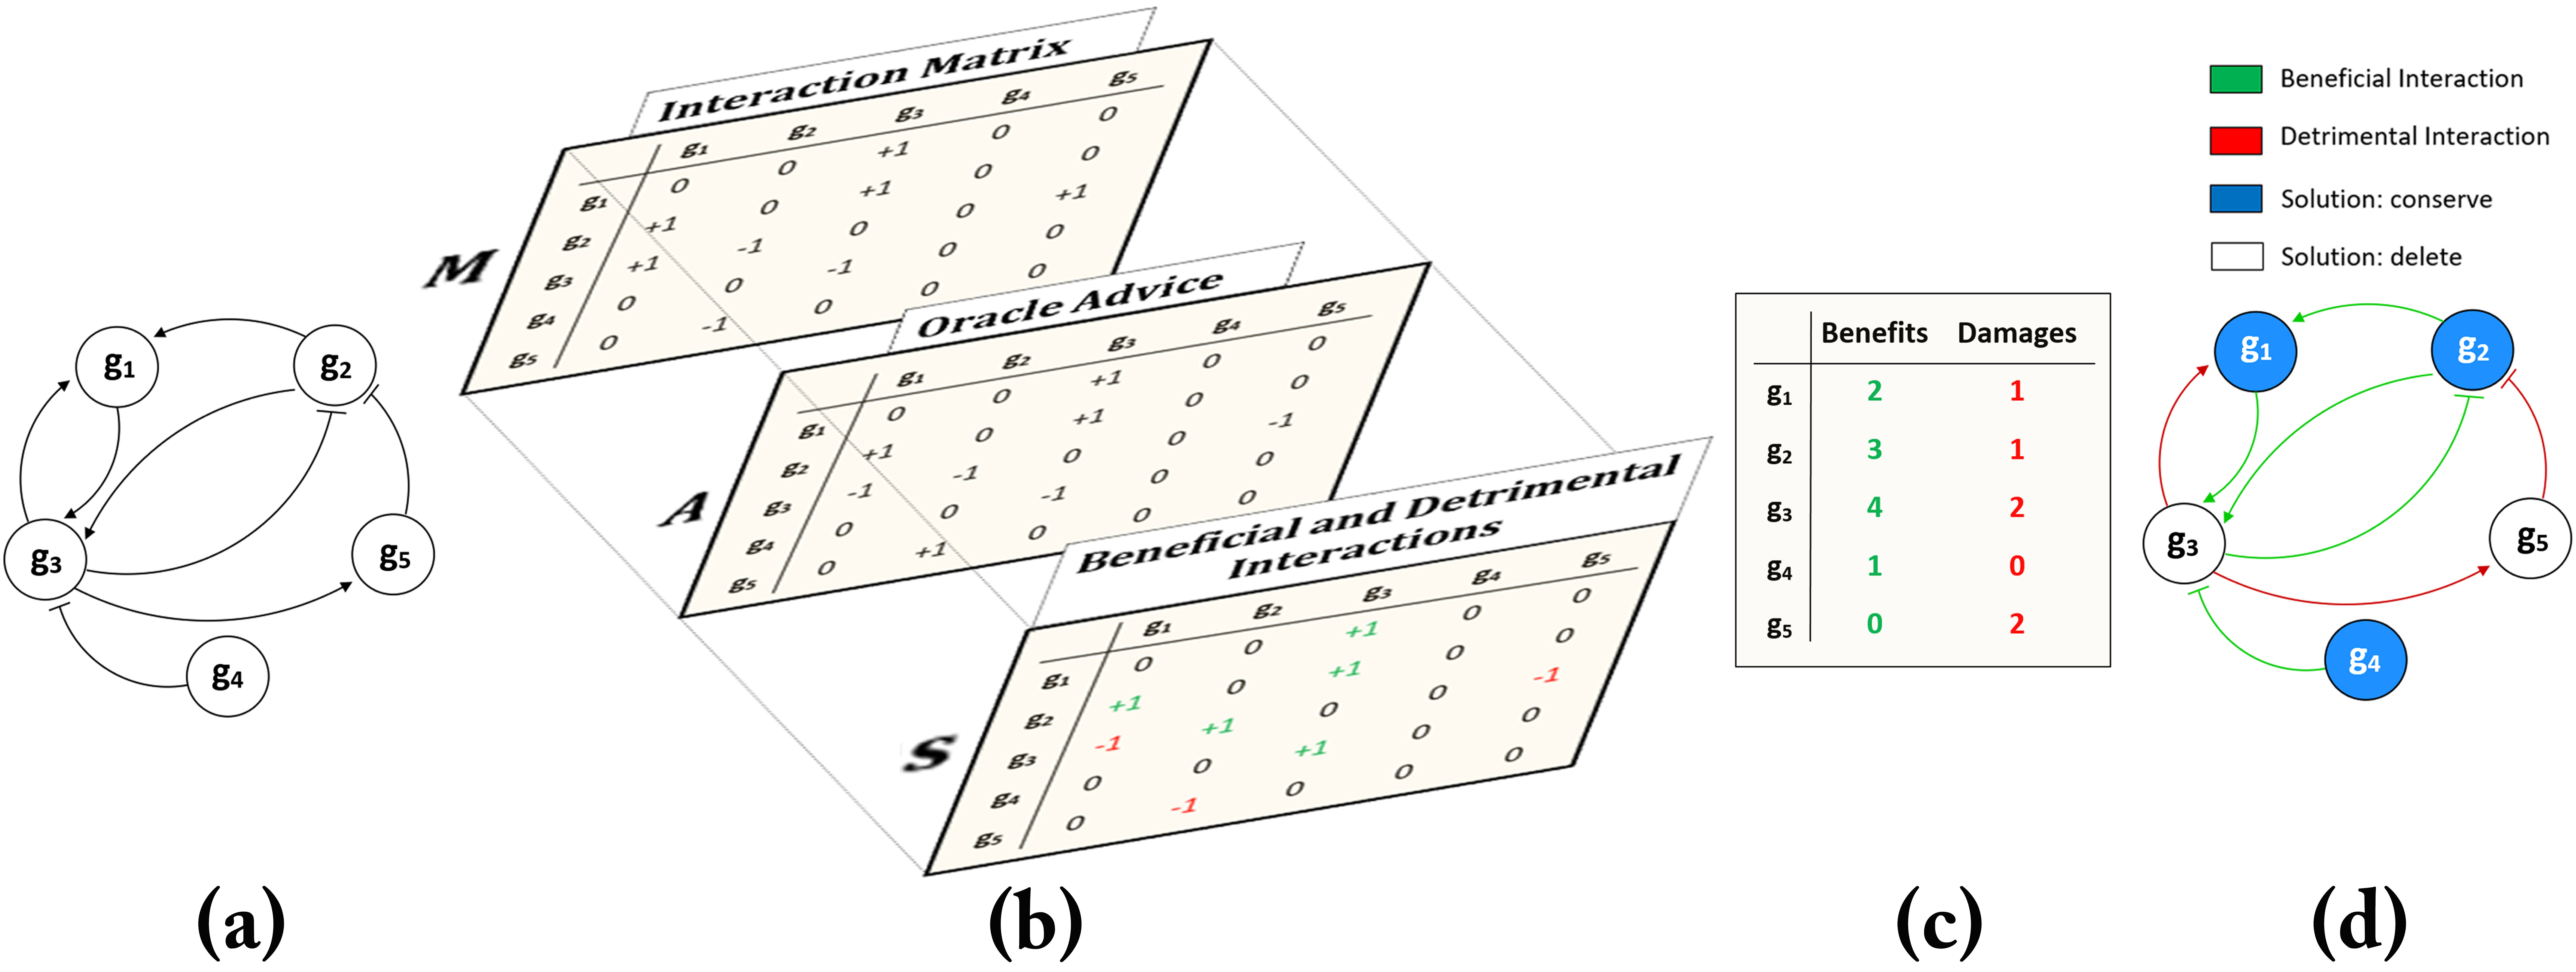
\includegraphics[width=1.0\textwidth]{/intro/photoshop/bigger_matrices.jpg} % original width= 42.65cm,  height = 19.86cm
		\caption{The network evolution problem. (a) A hypothetical  molecular interaction network of five genes $g_1 \dots g_5$ with 
		some inhibitory or promotional interactions (bar- and arrow-terminated edges, respectively). 
		(b) An equivalent representation of the network as an adjacency matrix ($M$). An Oracle advice ($A$) matrix indicates what the interactions in $M$ should 
		ideally be. 
		For example the promotional interaction from $g_1$ to $g_3$ (from $g_3$ to $g_5$) is in agreement (disagreement) with what the 
		Oracle says that interaction should be. Beneficial (in agreement) and detrimental (in disagreement) interactions are 
		shown in the bottom matrix $S$ in which $s_{jk}$ obtained by multiplying each $m_{jk}$ in $M$ with $a_{jk}$ in $A$. (c) Each gene $g_j$ in the network is 
		assigned a benefit (damage) value = the sum of beneficial (detrimental) interactions it projects onto 
		(out-edge, adding absolute values along along row $j$ in $S$) or attracts from (in-edge, adding absolute values along along column $j$ in $S$) other genes. 
		(d) Genes $g_4$, $g_5$ are unambiguous (totally beneficial, i.e. damage=0, or totally detrimental, i.e. benefit=0), while $g_1,g_2$ and $g_3$ 
		are ambiguous (having both non-zero benefit/damage scores). Assuming a threshold 2 tolerable detrimental interactions, the optimal evolutionary trajectory would be to conserve $g_1$,$g_2$ and $g_4$ and delete $g_3$ and $g_5$. }
\label{intro_figure}
\end{figure*}	
The benefit (damage)
score of each gene $g_j$, given an OA, is the sum of beneficial (detrimental) interactions that $g_j$ is
\textit{projecting} onto (out-edges) or \textit{attracting} from (in-edges) other genes. More precisely, the benefit score of $g_j$ is defined as:

 $b_j = \sum\limits_{k=1}^{n} m_{jk} \oplus a_{jk} \hspace{0.1cm}+\hspace{0.1cm} \sum\limits_{k=1}^{n} m_{kj} \oplus a_{kj} \quad\textrm{where:}$ 
 
 $\hspace{2cm}m_{xy} \oplus a_{xy}  =	\scriptscriptstyle{\begin{cases}	% in math mode, use scriptstyle/scriptscriptstyle, not small/tiny
											1 & \quad\textrm{if}\quad m_{xy} \times a_{xy} >0 \\
											0 & \quad\textrm{otherwise} 
									\end{cases}	
									}$
 
\vspace{.5cm}
and similarly the damage score is:
\vspace{.5cm}

$d_j = \sum\limits_{k=1}^{n} m_{jk} \ominus a_{jk} \hspace{0.1cm}+\hspace{0.1cm} \sum\limits_{k=1}^{n} m_{kj} \ominus a_{kj} \quad\textrm{where:}$ 

$\hspace{2cm}m_{xy} \ominus a_{xy}  = \scriptscriptstyle{\begin{cases}	% in math mode, use scriptstyle/scriptscriptstyle, not small/tiny
											1 & \quad\textrm{if}\quad m_{xy} \times a_{xy} < 0 \\
											0 & \quad\textrm{otherwise} 
									\end{cases}	
									}$

\vspace{.5cm}
An organism is clearly better off conserving a gene $g_j$ if its benefit $b_j\neq 0$  and damage $d_j=0$,
and deleting $g_j$ if $d_j\neq 0$ and $b_j=0$. We refer to such genes as \textit{unambiguous}. 
Clearly a degree-1 leaf gene $g_k$ (i.e. it only interacts with one other gene) is always 
unambiguous. A degree-2 $g_k$ can have one of four possible ($b_k$,$d_k$) values: 00, 01, 10, 11 with each digit representing an 
interaction (edge) and 0 or 1 implying the interaction is beneficial or detrimental, respectively, and as such $g_k$ has a 50\%
chance of being unambiguous under a random OA (i.e. equal likelihood of an interaction being deemed beneficial or detrimental by the Oracle).
As the degree $d$ of $g_k$ increases linearly, the probability of it being unambiguous under some OA decreases exponentially (namely,  $prob. = 2^{1-d}$). The network evolution problem (NEP) is that of defining the following function $f$: 

\begin{align*}
\scriptsize {f:\boldsymbol{G}  \rightarrow \{0,1\} \mys \textrm{maximizing} \mys  \sum\limits_{j=1}^{n} f(g_j)\times b_j \mys\mys\textrm{s.t.} \mys\mys \Bigg(  \sum\limits_{j=1}^{n} f(g_j)\times d_j  \Bigg)  \leq \boldsymbol{t} }
\end{align*}

	\begin{table}[t] %h:here, t:top of page, b:bottom of page, more: http://tex.stackexchange.com/questions/35125/how-to-use-the-placement-options-t-h-with-figures
		%\setlength\arrayrulewidth{.1pt}\arrayrulecolor[HTML]{0a84f7} %https://en.wikibooks.org/wiki/LaTeX/Colors#Adding_the_color_package
		\scriptsize %\small \tiny, \scriptsize, \footnotesize, \small, \normalsize, \large, \Large, \LARGE, \huge, and \Huge.
			\setlength\cellspacetoplimit{4pt} % padding in table cells
			\setlength\cellspacebottomlimit{4pt} %padding in table cells
			\begin{tabular}{c|c}  % http://tex.stackexchange.com/questions/302960/modify-arraystretch-for-a-single-row-in-table
				\hline
					BN & Biological Network
				\\[.01cm] \hline
					mLmH & Majority-leaves Minority-hubs topology
				\\[.01cm] \hline
					OA & Oracle Advice
				\\[.01cm] \hline
					NEP & Network Evolution Problem
				\\[.01cm] \hline
				    RVnRS & Random Variation non-Random Selection
				\\[.01cm] \hline
			\end{tabular}
			\caption{Abbreviations}
			\label{abbrev}	
	\end{table}

NEP has previously been proved NP-hard \cite{atiia_computational_2017-1}. Figure \ref{intro_figure} (a) shows a hypothetical small interaction network of 5 genes, 
with promotional and inhibitory interactions denoted by arrows and bars, respectively. The network can equivalently be represented as an (adjacency) 
interaction matrix $M$ (top matrix in Figure \ref{intro_figure} (b)) where +1, -1 signify promotional, inhibitory interaction, respectively 
(notice $m_{jk}$=0  when no interaction exists 
between $g_j$ and $g_k$). Against a hypothetical OA matrix $A$ (middle matrix in Figure \ref{intro_figure} (b)), where $a_{jk}\neq 0$ indicates 
what the interaction  $m_{jk}\neq 0$ should ideally be, an interaction is deemed beneficial or detrimental (bottom matrix in Figure \ref{intro_figure} (b)) 
when $m_{jk}$ and $a_{jk}$ are in agreement  
(i.e. $m_{jk}\times a_{jk}=1$) or disagreement (i.e. $m_{jk}\times a_{jk}=-1$), respectively. 
The benefit (damage) score of $g_j$ is the sum of beneficial (detrimental) interactions it is projecting onto (adding up absolute values along row $j$) 
or attracting from (along column $j$) other genes as shown in Figure \ref{intro_figure} (c). 
Genes that have zero benefit or damage score (respectively $g_5$ and $g_4$ in this example) should unambiguously be conserved (deleted). However, among 
genes with non-zero benefit and damage scores, an optimization search is needed to determine the optimal action (conserve and delete) that maximizes 
(minimizes) the overall total number of beneficial (detrimental) interactions. 
Clearly the larger the number of such ambiguous genes, the harder the optimization task would be. Assuming a certain threshold of tolerable detrimental interactions = 2 
for example, the optimal RVnRS trajectory (Figure \ref{intro_figure} (d)) would be one that leads to the conservation of $g_1,g_2$ and $g_4$, and the deletion of $g_3$ and $g_5$. 

%
\subsection{Evolutionary Algorithm}\label{evo_alg}
Evolutionary pressure is simulated on a network by randomly generating OAs on all interactions. An evolutionary algorithm selects for networks that 
on average yield easier instances of the optimization problem. Instance difficulty is measured by (1) the percentage of genes that are unambiguous 
(benefit and/or damage = 0) and (2) the effective total benefits that are contributed by conserved genes in an optimal solution. Networks whose 
instances are easiest are considered fit, and a new generation of offspring networks are bred from the top performing networks. Offspring 
population are mutated before the next round of OA generation and instance evaluation starts. 
Figure \ref{workflow} depicts the workflow of the algorithm. Individuals in the population are BNs, represented by their interaction matrix $M$. 
Individuals begin with either an empty network or one with randomly assigned edges.
 Mutation  modifies connectivity between nodes by random edge reassignment to two randomly selected nodes, or by
 adding nodes and edges in simulations where network growth occurs. After mutation, the fitness of each network in the population is 
 assessed based on the computational 
ease of the NEP instances that result from applying repeated evolutionary pressure (multiple OAs) on the network.
 Exact replicas are generated from the fittest 10\% of the networks to create the next
population networks. %Over many generations networks adept at producing easier instances of NEP are selected for. 
For a network of $N$ nodes, the unambiguity metric $U$ emphasizes sparsely connected nodes and is defined as the ratio of unambiguous nodes relative to 
the total number of nodes: 

\begin{align*}
U=\frac{|\{g_i:b_i=0|d_i=0\}|}{N}
\end{align*}

The solution vector to an NEP instance is a sequence $(s_1, s_2, .., s_k)$ where $s_i\in\{0,1\}$ 
and $s_i=1 \mys (s_i=0)$ implies "conserve" ("delete").
Accumulated benefits in an NEP instance's optimal solution is a multi-set $B=\{b_i: s_i=1\}$, and the 
effective accumulated benefits $B_e=sum(set(B))$ (i.e. $B_e$ is $B$ normalized by the number of genes it takes 
to contribute a certain benefit value). For example, with $B1=\{1,1,1,2\}$ and $B2=\{2,3\}$, $sum(B1)=sum(B2)$,  but $B1_e=3$ while $B2_e=5$. 
$B_e$ reflects the effort (no. of genes conserved) needed to achieve a certain benefit. Generally, with
a gene of degree $d$ and assuming all its in- and out-edges are in agreement with the OA (i.e. a totally
beneficial gene), it would single-handedly contribute $|d|$ to $B_e$. In the opposite extreme, if such a gene were broken into $n$ specialty genes with degrees
$(d_1, d_2.., d_n), d_i=1 \forall i$, then $B_e$ reduces down to $1$  ($(d_1 + d_2\dots d_n)\div n$) assuming all such genes are beneficial. Let $B_{tot}$ be the total benefit in a given NEP instance (the sum of gained benefits of conserved genes and lost benefits of deleted genes), the fitness of a given NEP instance $S$ is measured as:

\begin{align*}
F(S) = U^\alpha \times \frac {B_e}{B_{tot}}
\end{align*}

where $\alpha\in \approx \mathbb{R}^{+}$. In all simulations, we used $\alpha=2$, which calibrated the opposing effects \cite{kim_positive_2007} 
of the the two selection criteria (instance size in $U$ and effective total benefit in $\frac {B_e}{B_{tot}}$, 
further discussed in \ref{adapt_section} and Figure \ref{adap_fig}). 
The larger a gene's degree is the more ambiguous it can be. Unambiguous genes do not need to be included in the 
computationally costly optimization search and can $a priori$ be deemed beneficial (detrimental) and should therefore be 
conserved (deleted) regardless of the state of other genes. Mutations on unambiguous nodes will have a clear selection 
gradient since they are more likely to be totally beneficial or totally detrimental but not both. 
Although the problem is generally NP-hard, instances with small effective instance size (large number of unambiguous genes) 
are easier to satisfy. 
Clearly a very sparse network results most genes being unambiguous, but it also leads to an explosion of genome size
since more genes are needed to fulfill a function that could have been handled by a single hub gene. 
While $B_e$ measures the ability of a network to capture more benefits with less genes to conserve, 
normalizing it by the total benefits $B_{tot}$ discourages networks that hemorrhage a large number of possible benefits lost to deleted genes.
\begin{figure}[H]
		\centering
		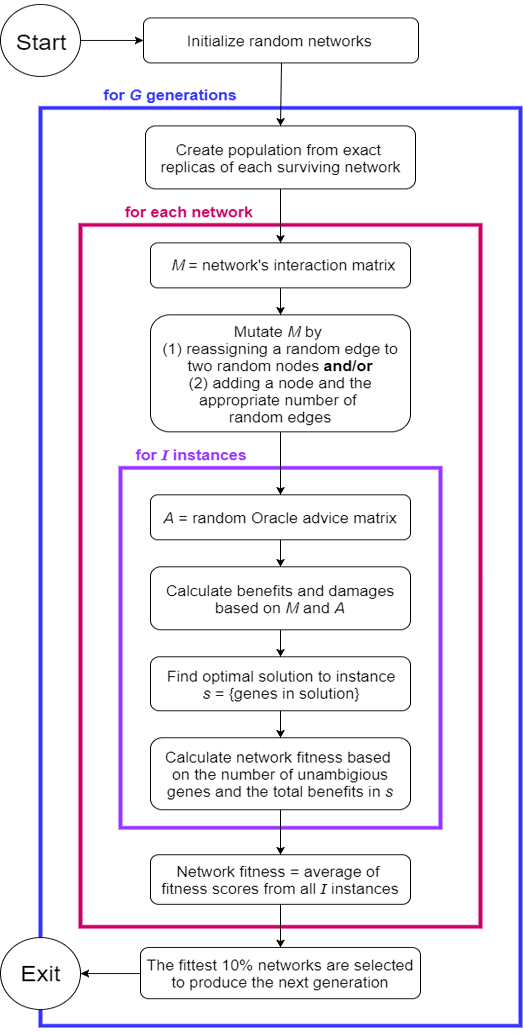
\includegraphics[scale=.42]{workflow/workflow_transparent_2nd_draft.png} % original width= 42.65cm,  height = 19.86cm
		\caption{The algorithmic workflow of the evolutionary algorithm. 
		Simulations begin with empty networks or seed networks that have randomly distributed edges. 
		Each network is randomly mutated by reassigning one edge at each generation and,  
		if growth is allowed, one node is also added along with as many randomly 
		assigned edges as needed to maintain the desired edge:node ratio. 
		An instance of the network evolution problem (NEP) is obtained by generating a random Oracle advice (OA) on all edges in the network. 
		A network's fitness at each instance $S$ is calculated following the $F(S)$ formula (Section \ref{evo_alg}).
		The 10\% of networks with the highest average fitness over all instances are selected to breed a population of networks for the subsequent generation.}
		\label{workflow}
\end{figure}
%	\printbibliography
%\end{document}
%end_custom_content
\section{Results}
\subsection{Adaptation}\label{adapt_section}
	A population of random 400-node seed networks, each having an edge:node ratio matching that of the Yeast network (Table \ref{networks_summary})\footnote{The real BNs used in this study (Table \ref{networks_summary}) are publicly available in: \url{http://cs.mcgill.ca/~malsha17/permlink/acmbcb17/}}, 
	is subjected to successive rounds  of RVnRS. 
	The evolutionary algorithm mutates each network in the population by edge-reassignment only and subsequently 
	selects the fittest networks (according to their $F(S)$ values) to breed the next population of networks.
	The networks are sorted according to fitness, and the top 10\% are selected. 
	Replicas are produced from each selected network bringing the population to its previous size. Figure \ref{adap_fig} (a) displays 
	the degree distribution of the fittest adapted network after 2000  mutate-select-breed generations (black dots) against 
	100 400-node randomly sampled subnetworks from Yeast. 
	The connectivity of of the adapted network morphed into the mLmH property matching that of Yeast. 
	Figure \ref{adap_fig} (b) shows the change in the overall 
	fitness score of the fittest network in the population at each generation (top) as well as the change in fitness score per metric 
	($U^2$ (left) and $\frac {B_e}{B_{tot}}$ (right) subplots). The fitness improves dramatically at the beginning and plateaus by generation 2000. 
	The remaining fluctuations are largely due to variance in NEP as different instances may vary in fitness for the same network. 
	$U$ and $\frac {B_e}{B_{tot}}$ are balance the two competing forces of selecting for unambiguity (leaf nodes) and effective total benefits (hub nodes). 

	Figure \ref{adap_fig} (c) depicts the percent of unambiguous nodes at the beginning and end of the simulation. The adapted network at generation 2000 
	has more leaf nodes contributing to the unambiguous 100:0 and 0:100 $benefit$:$damage$ ratio groups. The random network exhibits 35.9\% unambiguous nodes (solid red and green slices), whereas 
	the evolved network results in 53.5\% unambiguous nodes. The latter clearly produces NEP instances with small effective instance sizes. 
	Figure \ref{adap_fig}(d) portrays the composition of the NEP solution. Adapted networks fit larger hubs into the solution due to 
	the fact that the more leaf nodes a network has the less threshold damage is consumed and therefore hubs (which are likely to 
	carry damaging interactions) are more likely to  be conserved (i.e. part of the optimal solution) for their benefits and despite their damages. 
	That implies that a hub involved in damaging interactions 
	can still be tolerated while more experimentation in network composition (conserve/delete) and/or connectivity (mutations that 
	affect interaction affinity) can take place \cite{kim_positive_2007}. 
	Figure \ref{adap_fig} (e)  
	displays the change in degree distribution on a normal and a log-scaled (inset) plot. The seed networks at 
	the first generation are created by randomly assigning edges resulting in an 
	exponential degree distribution centred around the average degree. In stark contrast, adapted networks at generation 2000
	display a heavy-tailed distribution with a few highly
	connected hubs. The model robustly evolves to mLmH topology despite unfavourable starting conditions. Very low degree (leaf) nodes dramatically increase in 
	frequency, while more high-degree (hub) nodes emerge. 
%
\subsection{Adaptation with Growth}\label{evolution_results}
	The same evolutionary algorithm is applied starting from a near empty seed network that grows in size
	over the generations. Networks in the population start with 4 nodes and periodically acquire new nodes 
	and edges. Figure \ref{evol_figure} illustrates simulated networks and their corresponding
	BNs that have the same edge:node ratio. The BNs are protein-protein interaction networks of 6 different organisms. The simulation is terminated when the simulation network
	reaches the size of 400 nodes. For comparison, 
	 100 400-node subnetworks are sampled from the corresponding BN (colour dots in Figure \ref{evol_figure}). 
	 The degree distributions of simulated networks (black dots in Figure \ref{evol_figure})
	closely match their corresponding BNs. 
	%The simulation also replicates the tendency  for BNs to increase leaves at lower edge to node ratios. 
	%Sampled subnetworks from BNs may include larger hubs, since larger networks have more edges to produce highly connected nodes. 
	The frequency of hubs in  networks sampled from real BNs is comparable to those resulting from simulations, although the latter have lower probability of generating
	extremely highly connected hubs given their smaller size.  
\begin{comment}
Fitness is based on a leaf metric that emphasizes sparsely connected nodes and a hub metric that promotes highly connected nodes. Fitness is the product of these two forces, which stretch the degree distribution in both directions to exhibit heavy-tailed connectivity. 

$f(N)=LF \times HF$

The leaf metric is based on minimizing the correlation between benefits and damages. Previous work demonstrates that higher correlation between values and weights result in more computationally expensive knapsack problems \cite{pisinger_where_2005}. Nodes are evaluated based on the ratio of benefits to all interactions (benefits + damages). The symmetrical case of damages to all interactions is also considered, and the higher outcome is preferred. Lower degree nodes are far more likely to be uncorrelated. The ratio alone vastly prefers degree one, so the square root of the ratio is taken to create smoother spectrum. The total leaf fitness is the average of the fitness of all nodes. 

$LF = \frac { |\{g_i: b_i = 0 | d_i=0\}| }  {|G|}$

The hub metric captures the ability to garner more benefits with less change. The benefits of the nodes in solution to the NEP is transformed from a multi set to a single set, which removes redundant numbers. The hub metric is composed of the sum of the single set of the benefits in the solution, divided by the sum of the multi set of benefits in the solution. Since the solution tends to include many small elements, the metric evaluates the proportion of the solution that is due to large, infrequent elements.

$HF = \frac { |\{g_i: b_i = 0 | d_i=0\}| }  {\sum\limits_{i=1}^{n} b_i}$
\end{comment}
\setlength{\textfloatsep}{0pt plus 1.0pt minus 1.0pt} % http://tex.stackexchange.com/questions/26521/how-to-change-the-spacing-between-figures-tables-and-text
	\begin{table}[t] %h:here, t:top of page, b:bottom of page, more: http://tex.stackexchange.com/questions/35125/how-to-use-the-placement-options-t-h-with-figures
		%\setlength\arrayrulewidth{.1pt}\arrayrulecolor[HTML]{0a84f7} %https://en.wikibooks.org/wiki/LaTeX/Colors#Adding_the_color_package
		\scriptsize %\small \tiny, \scriptsize, \footnotesize, \small, \normalsize, \large, \Large, \LARGE, \huge, and \Huge.
			\setlength\cellspacetoplimit{4pt} % padding in table cells
			\setlength\cellspacebottomlimit{4pt} %padding in table cells
			\begin{tabular}{c|c|c|c}  % http://tex.stackexchange.com/questions/302960/modify-arraystretch-for-a-single-row-in-table
				\hline\hline
					\textbf{Network} & \textbf{no. nodes} & \textbf{no. edges}	& \textbf{edge:node ratio}
				\\[.05cm] \hline
					Plant \cite{consortium_evidence_2011}  & 2402 & 5486 & 2.3
				\\[.05cm] \hline
					Bacteria \cite{rajagopala_binary_2014} & 1014 & 1967 & 1.9
				\\[.05cm] \hline
					Yeast \cite{yu_high-quality_2008}      & 1647 & 2682 & 1.6
				\\[.05cm] \hline
					Worm \cite{simonis_empirically_2009}   & 2214 & 3659 & 1.7
				\\[.05cm] \hline
					Fly \cite{vinayagam_integrating_2014}  & 3058 & 5930 & 1.9
				\\[.05cm] \hline
					Human \cite{yang_widespread_2016}      & 473  & 885 & 1.9
				\\[.05cm] \hline
				    Bacteria Regulatory \cite{gama-castro_regulondb_2016} & 898 & 1481 & 1.6
				\\[.05cm] \hline
				    Mouse Regulatory \cite{liu_regnetwork:_2015} & 1436 & 3673 & 2.6
				\\[.05cm] \hline\hline
			\end{tabular}
			\caption{Summary of real biological networks against which simulations were conducted with references to their sources. Bacteria Regulatory and Mouse Regulatory
			 involve transcription-factor (TF)-gene, TF-TF or small RNA-gene interactions, while all other networks involve protein-protein interactions. 
			         }\label{networks_summary}	
	\end{table}
\begin{figure*}[t]
		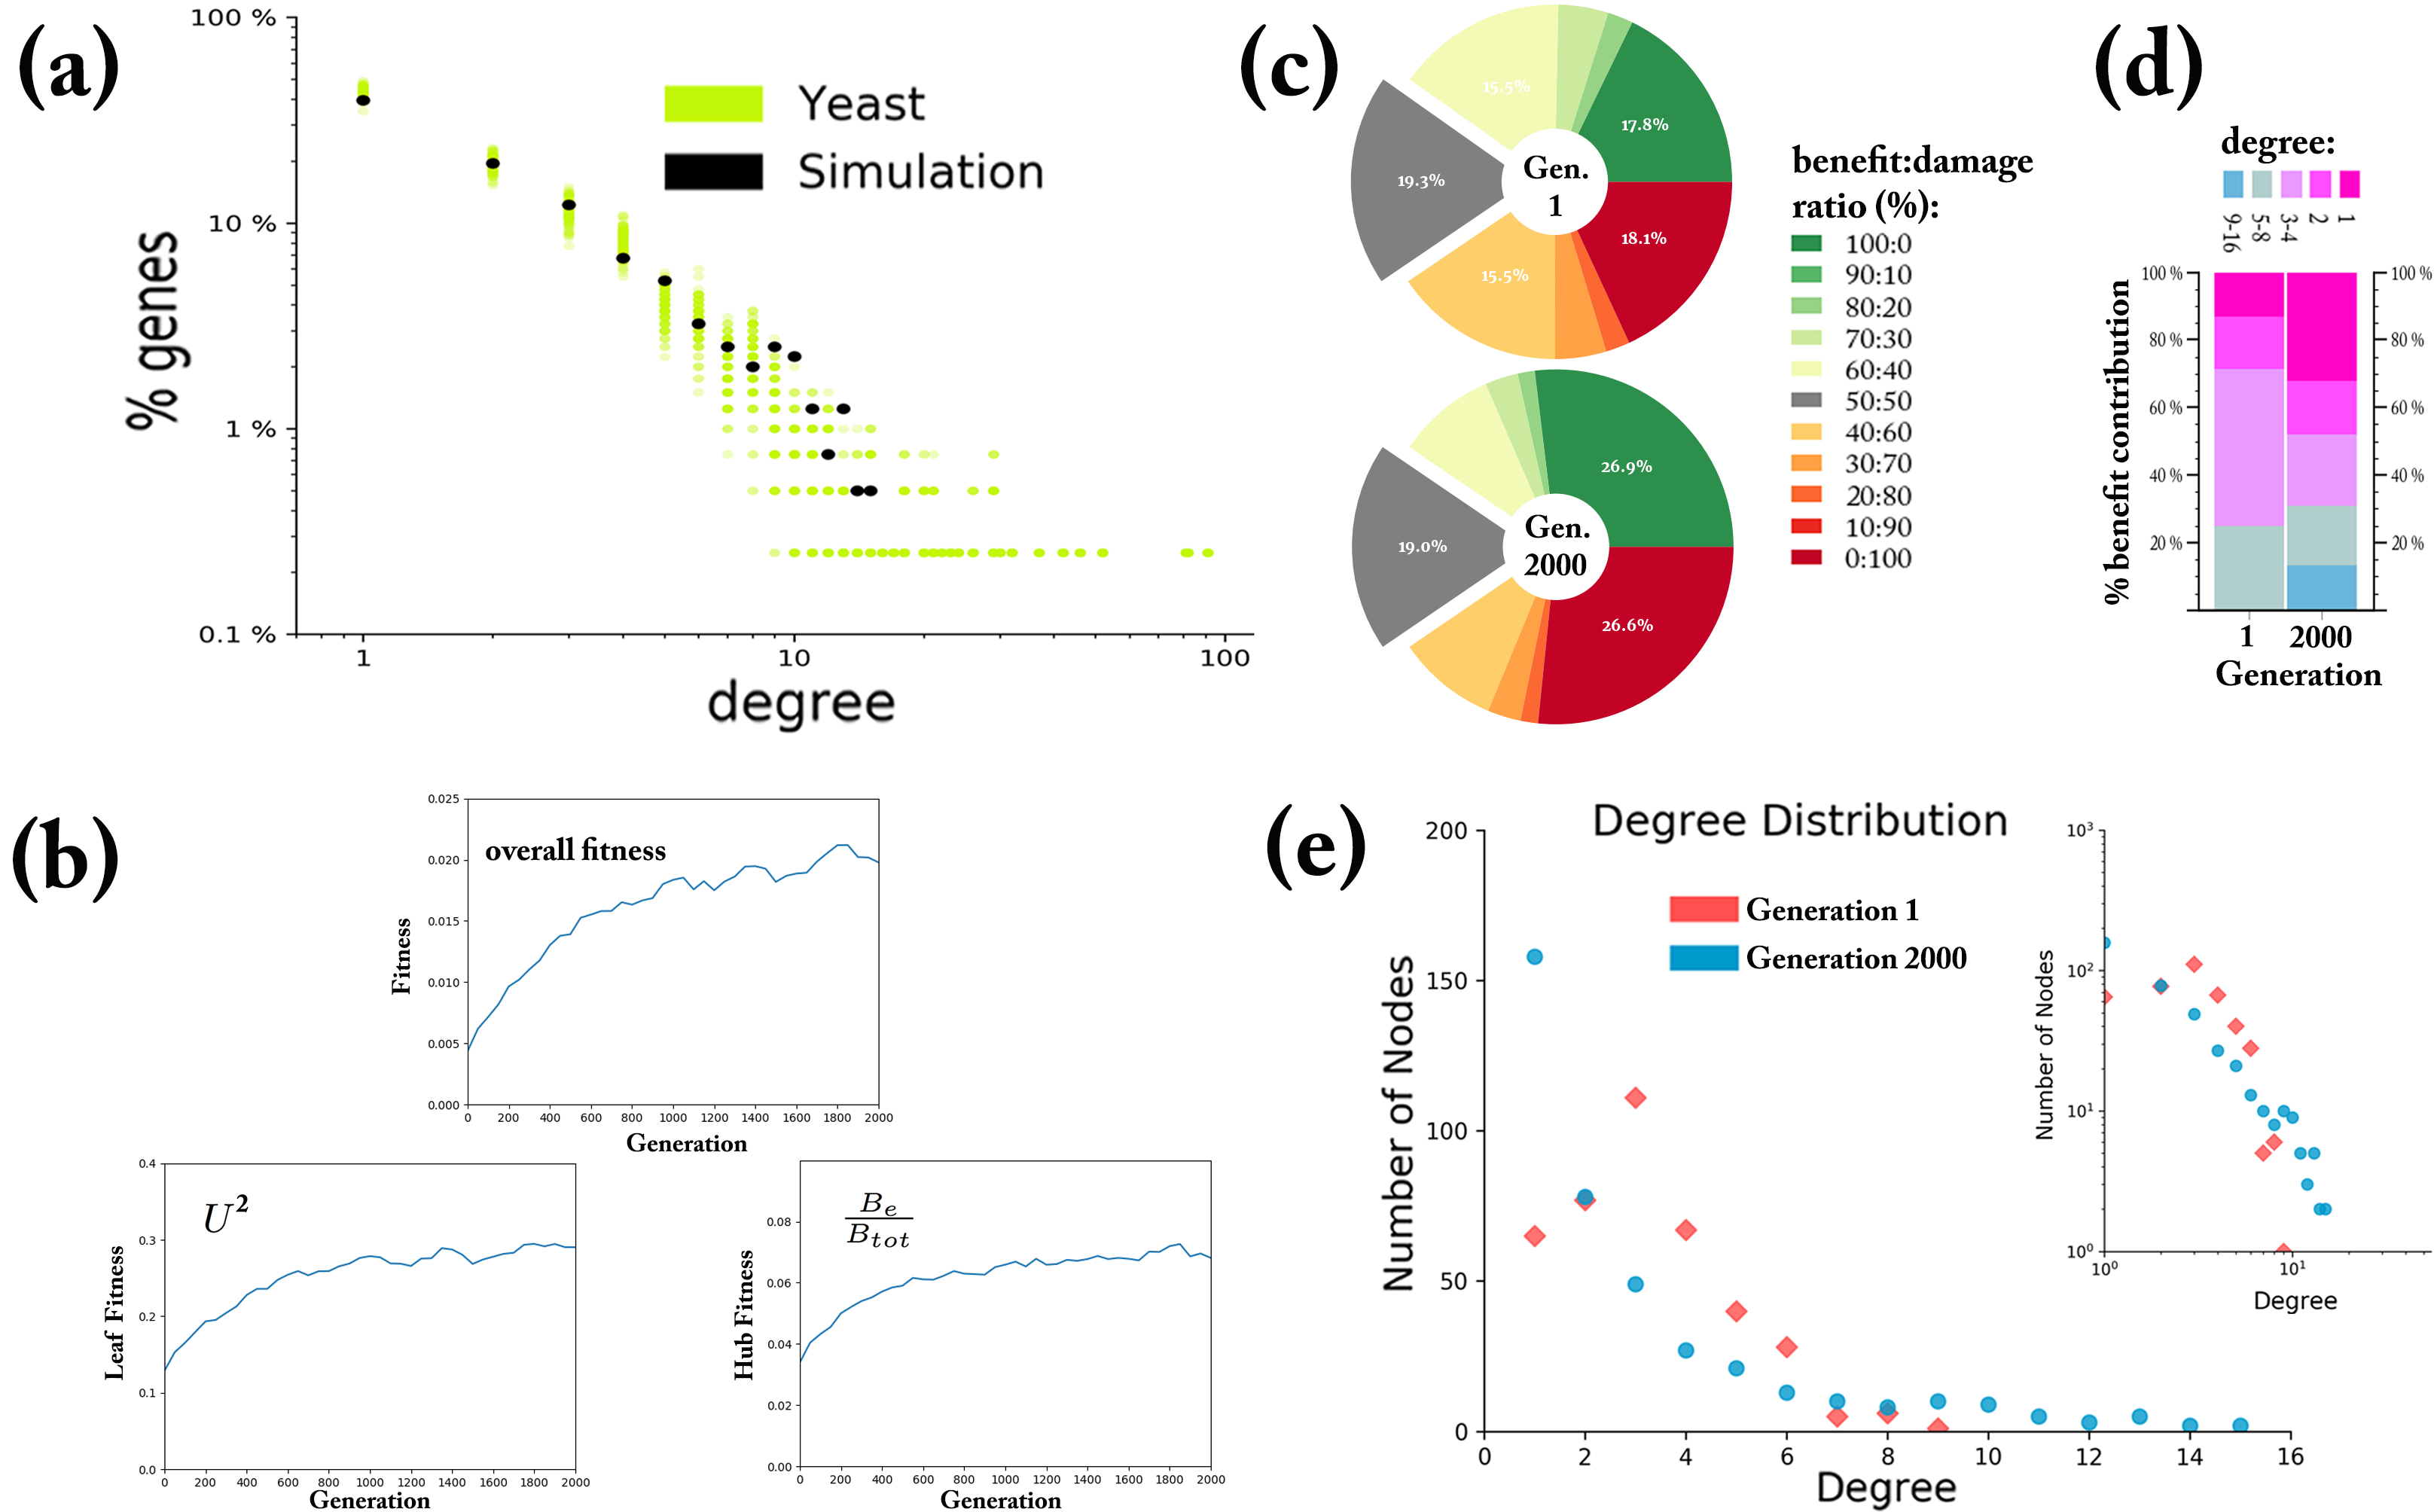
\includegraphics[scale=.65]{/adaptation/photoshop/processed_v5.png}
		\caption{Adaptation of a random seed network. 
					(a) starting from a network with the same  edge:node ratio as the Yeast network, but with edges randomly assigned to nodes, the mLmH property emerges after 2000 generations of random mutation (random edge re-assignment) and random selection according to instance size and effective total benefits.
					(b) Improvement in fitness over the generations.  The overall, $U$-only, and $\frac {B_e}{B_{tot}}$-only  fitness per generation depicted in top, bottom-left, bottom-right subplots respectively. 
					(c) The percentage of unambiguous genes in NEP increases over the course of simulated adaptation, resulting in easier instances with smaller effective instance sizes. Solid green (red) slices represent nodes with  zero damage and non-zero benefit (zero benefit and non-zero damage). Top pie: the initial random network at generation 1 includes on average 35.9\% unambiguous nodes; bottom pie: after 2000 generations, the network 
					has on average 53.5\% unambiguous nodes.
					(d) The percentage of benefits that nodes, grouped by degree range (legend, top), contribute to NEP solution before (generation 1 (left bar), random seed network) and after simulated adaptation (generation 2000, right bar). Larger nodes in adapted (generation 2000) network contribute a higher proportion of benefits due to the fact that the large number of damage-minimal leaves do not consume damage tolerance threshold thereby increasing the likelihood of (the more ambiguous and more tolerance-consuming) hubs to be in solution. The benefits in the solution for a random network  (generation 1) are predominantly contributed by medium degree nodes. After 2000 generations, a marked increase in the contribution by the majority leaves (degree 1 and 2 particularly) and by high degree hubs of degree $\geq$ 5 is observed. 
					(e) Initial random networks have exponential distributions. After simulated adaptation, mLmH topology emerges (more leaves and high-degree hubs in exchange for less medium-degree nodes);  inset: the same plot in log scale. 
		}
		\label{adap_fig}
\end{figure*}	

\begin{figure*}[t]
		\centering
		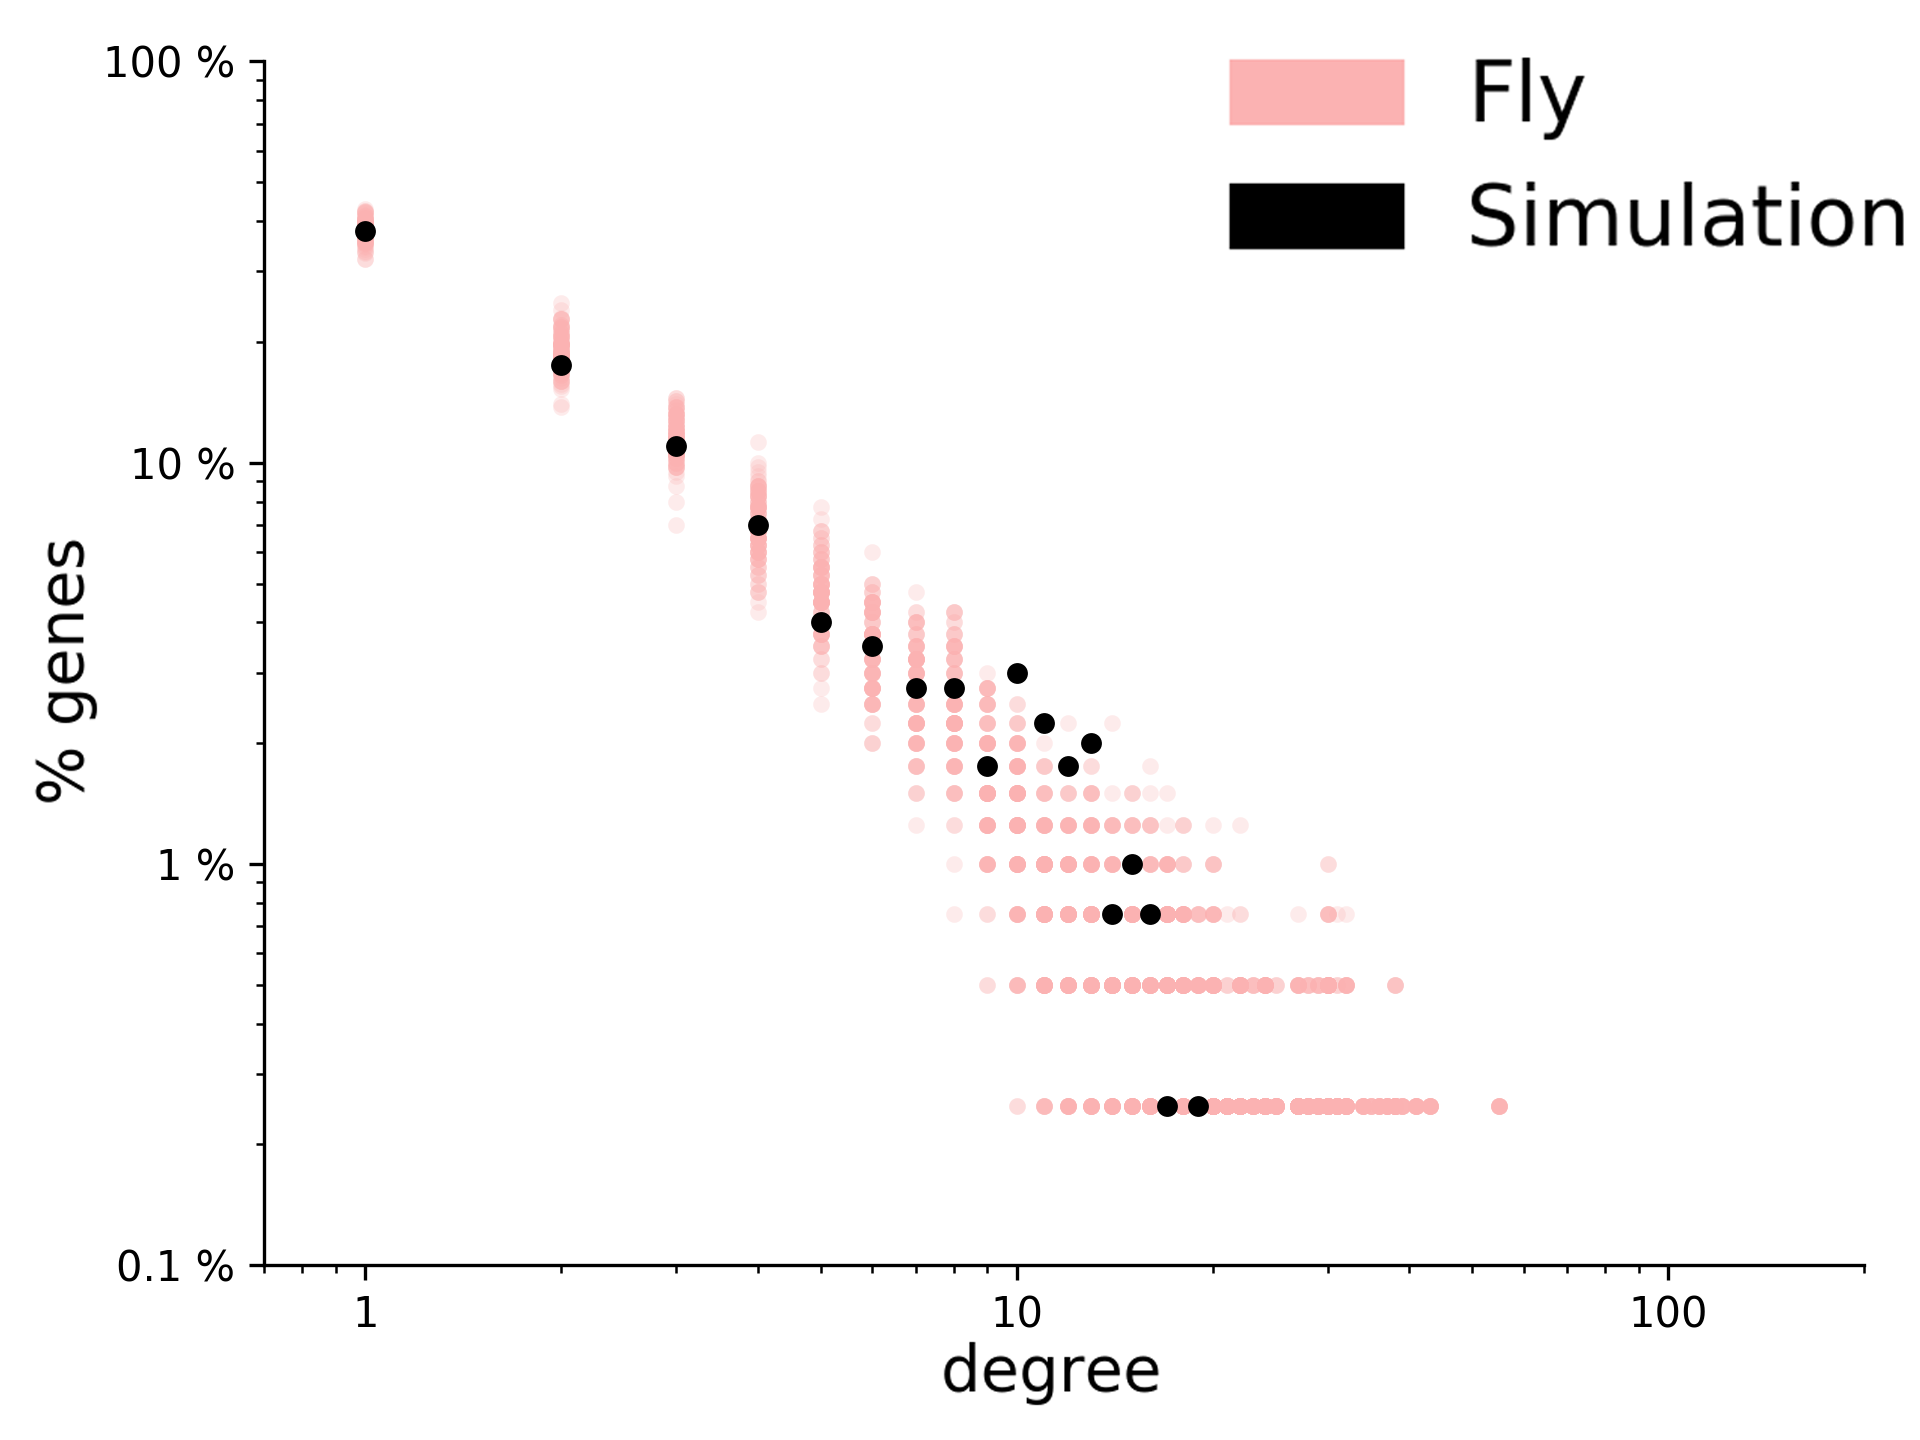
\includegraphics[scale=.36]{/adaptation_with_growth/faint_alpha/Evo_Fly.png}
		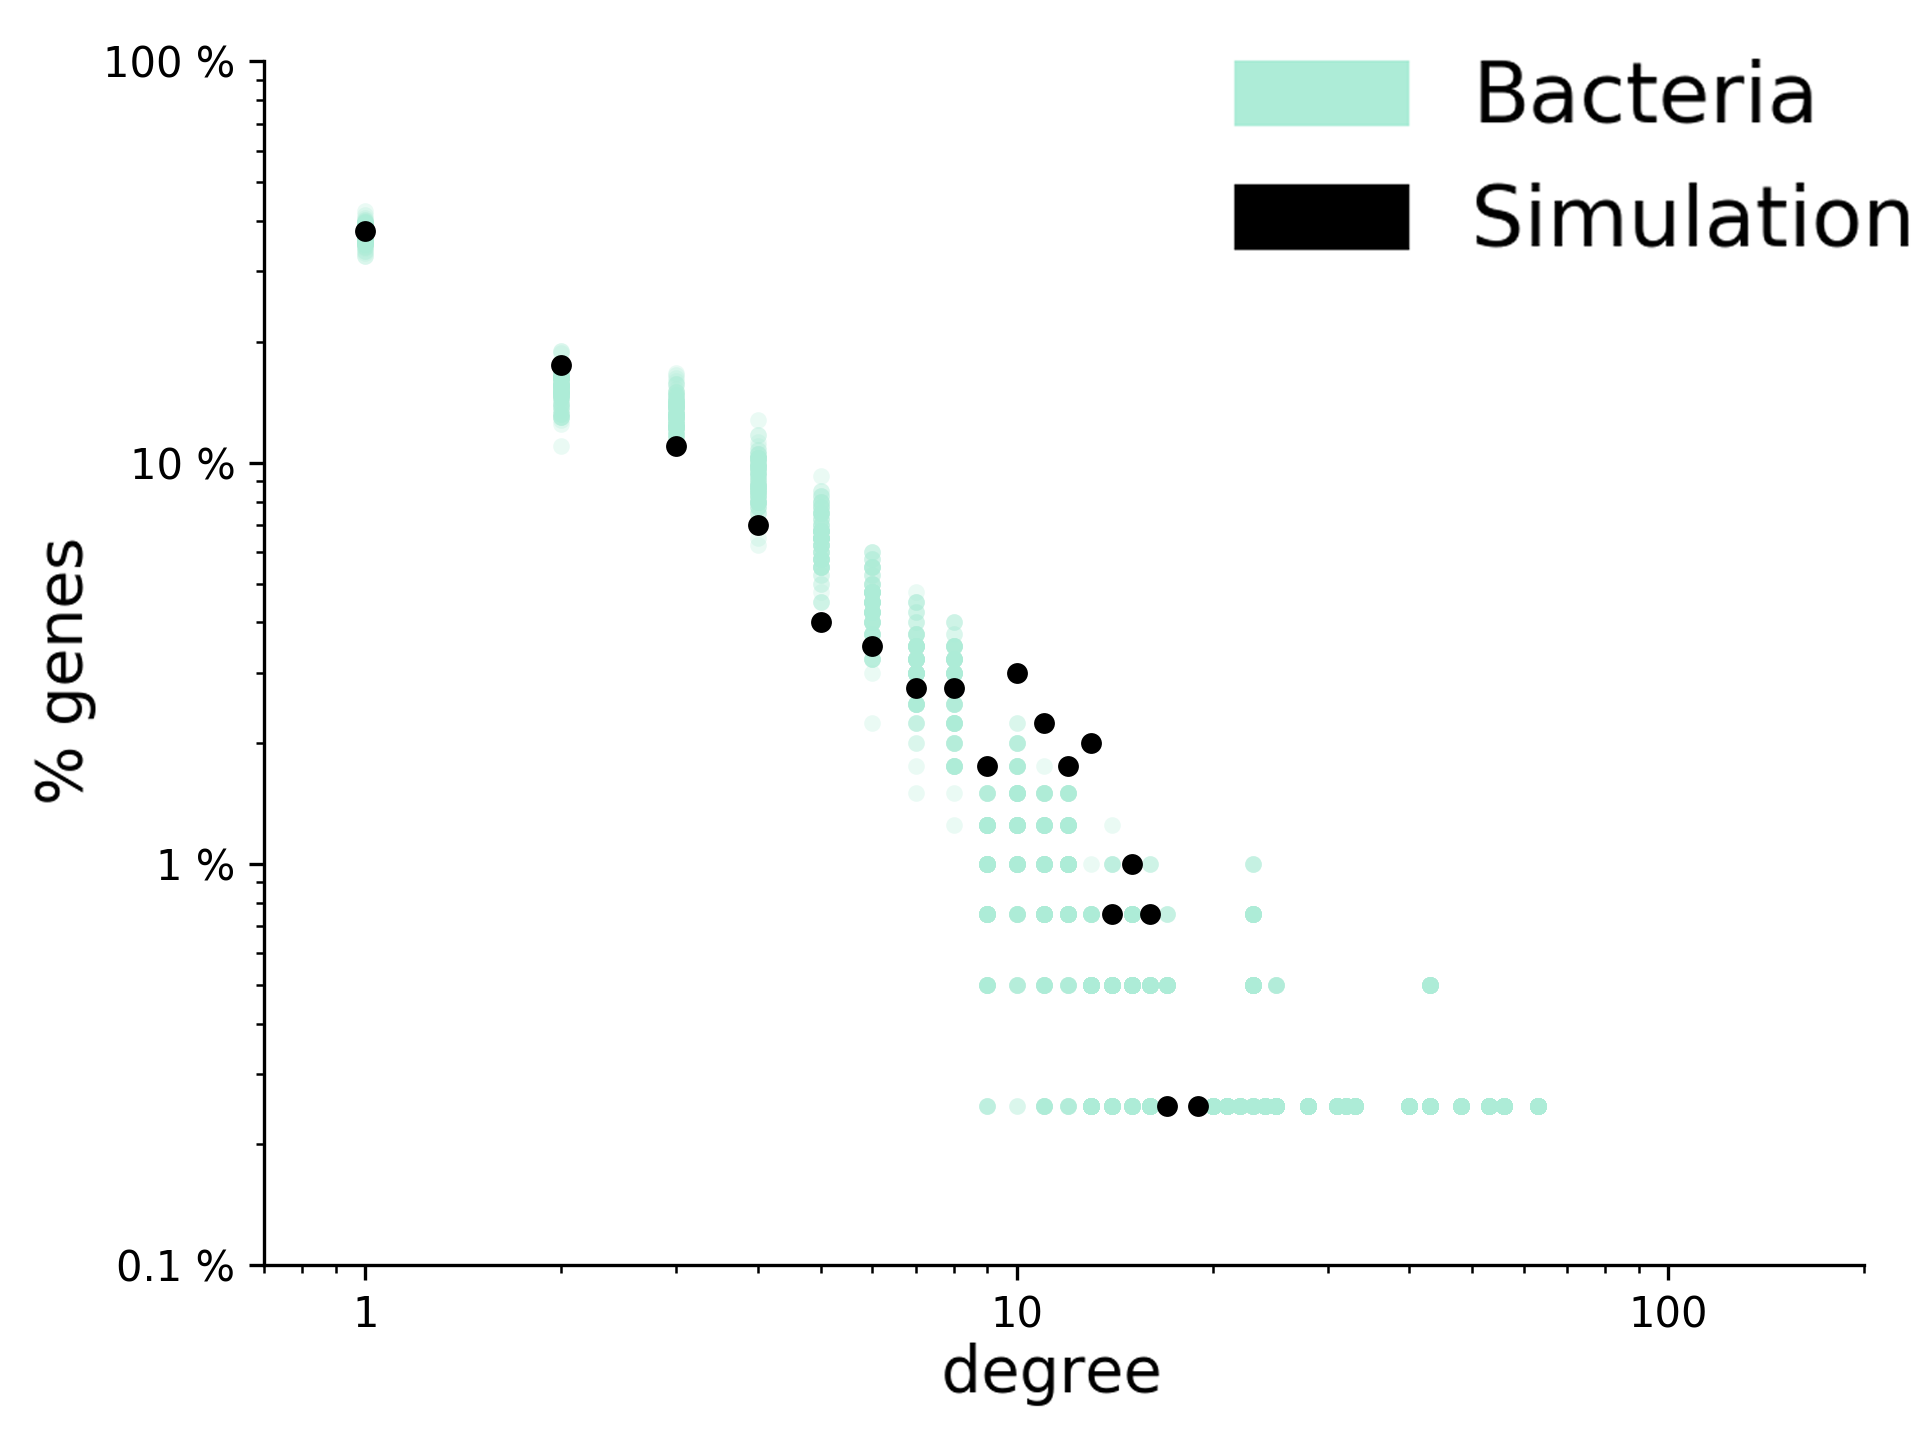
\includegraphics[scale=.36]{/adaptation_with_growth/faint_alpha/Evo_Bacteria.png}
		\includegraphics[scale=.36]{/adaptation_with_growth/faint_alpha/Evo_Humaniso.png}
		\\
		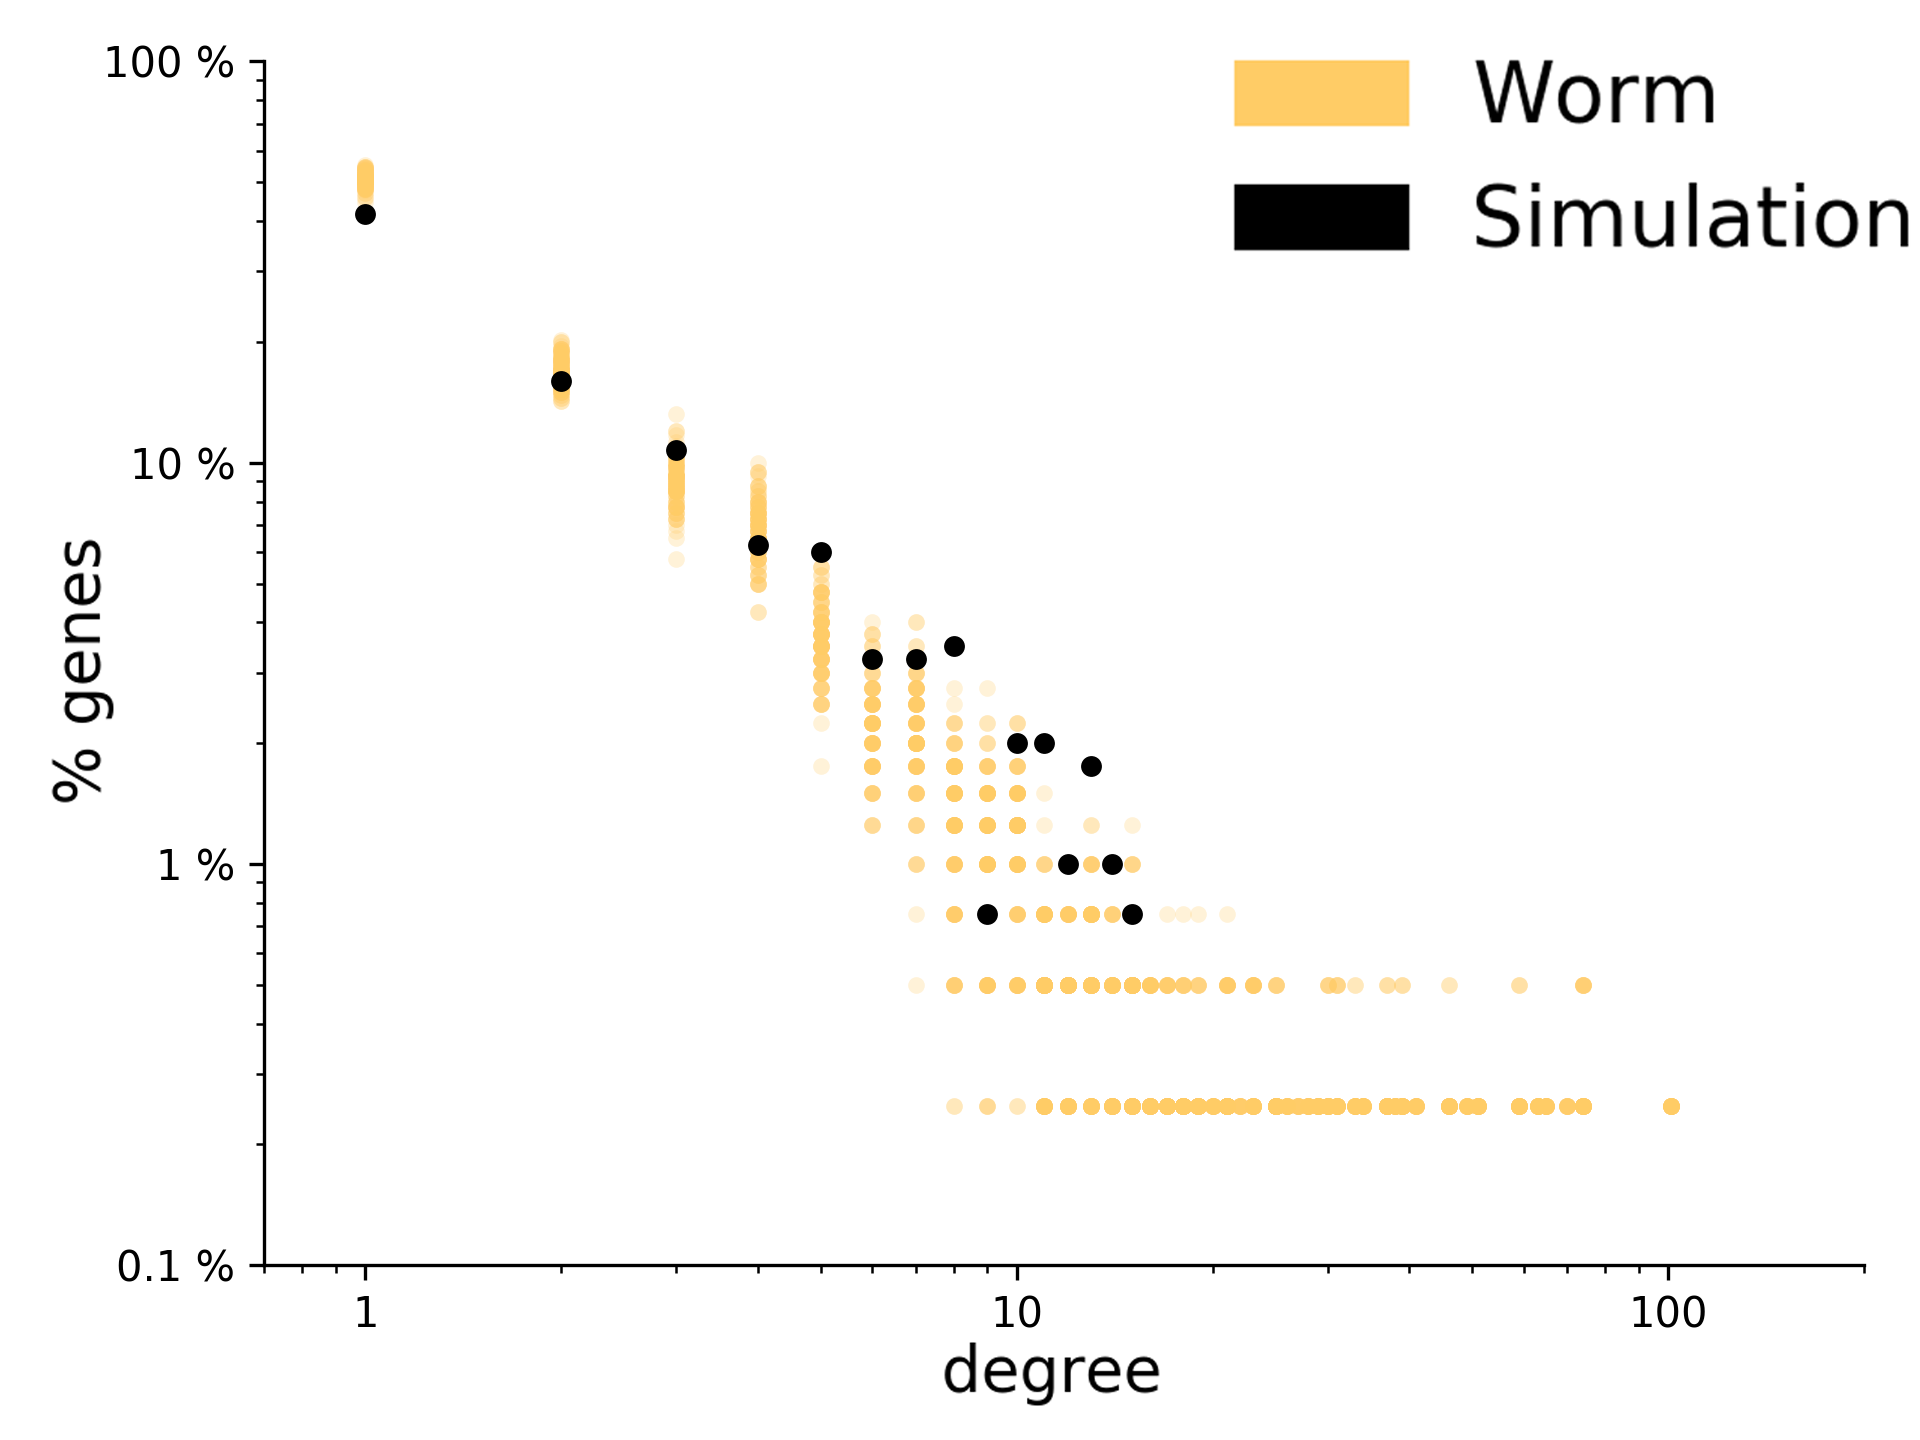
\includegraphics[scale=.36]{/adaptation_with_growth/faint_alpha/Evo_Worm.png}
		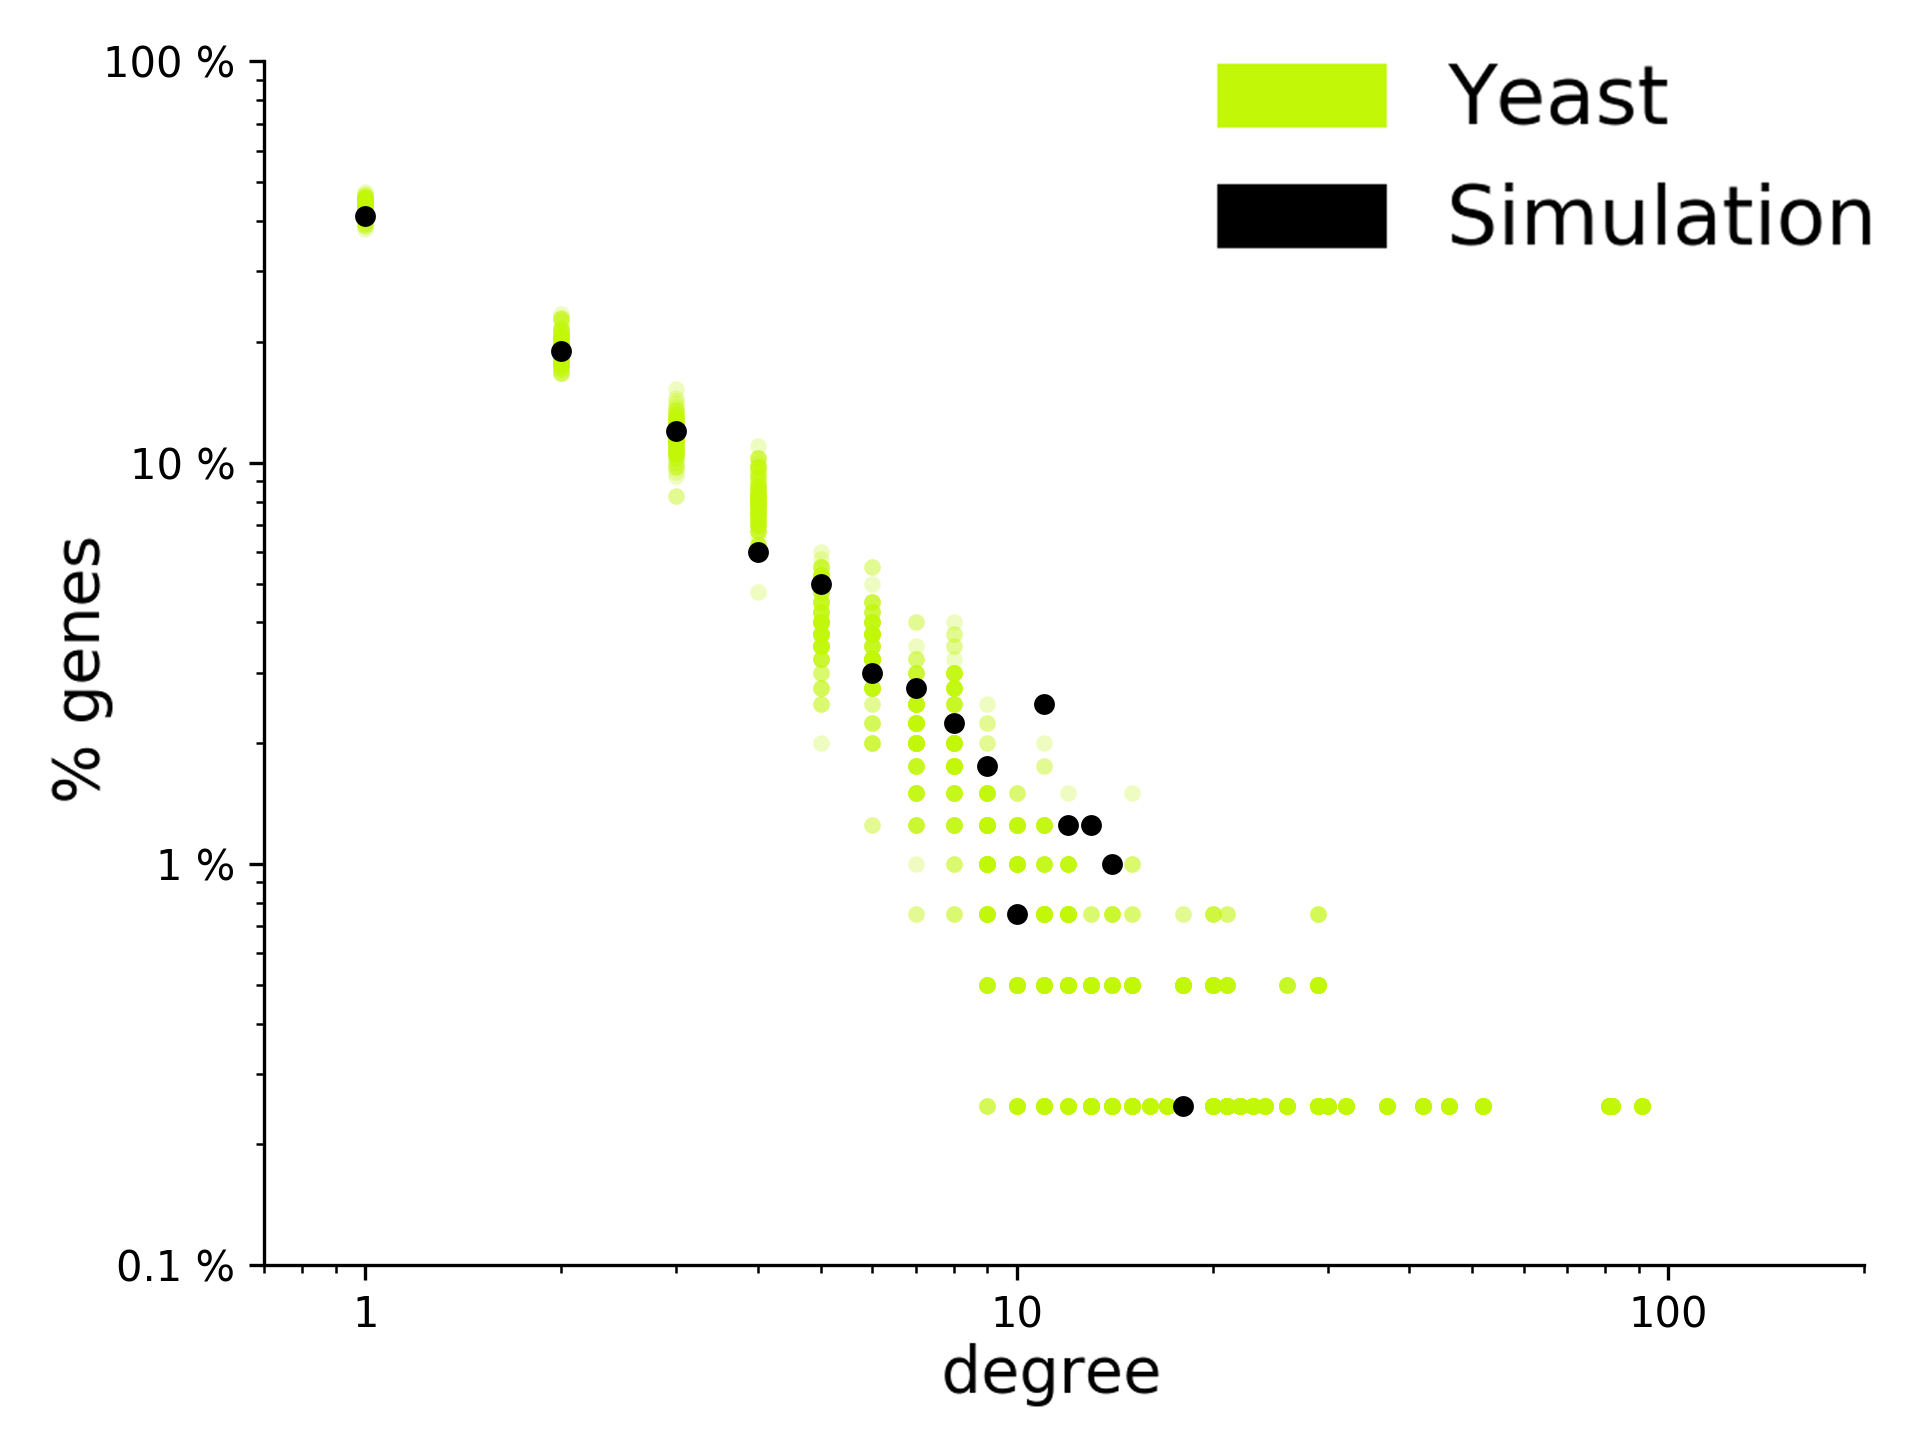
\includegraphics[scale=.36]{/adaptation_with_growth/faint_alpha/Evo_Yeast.png}
		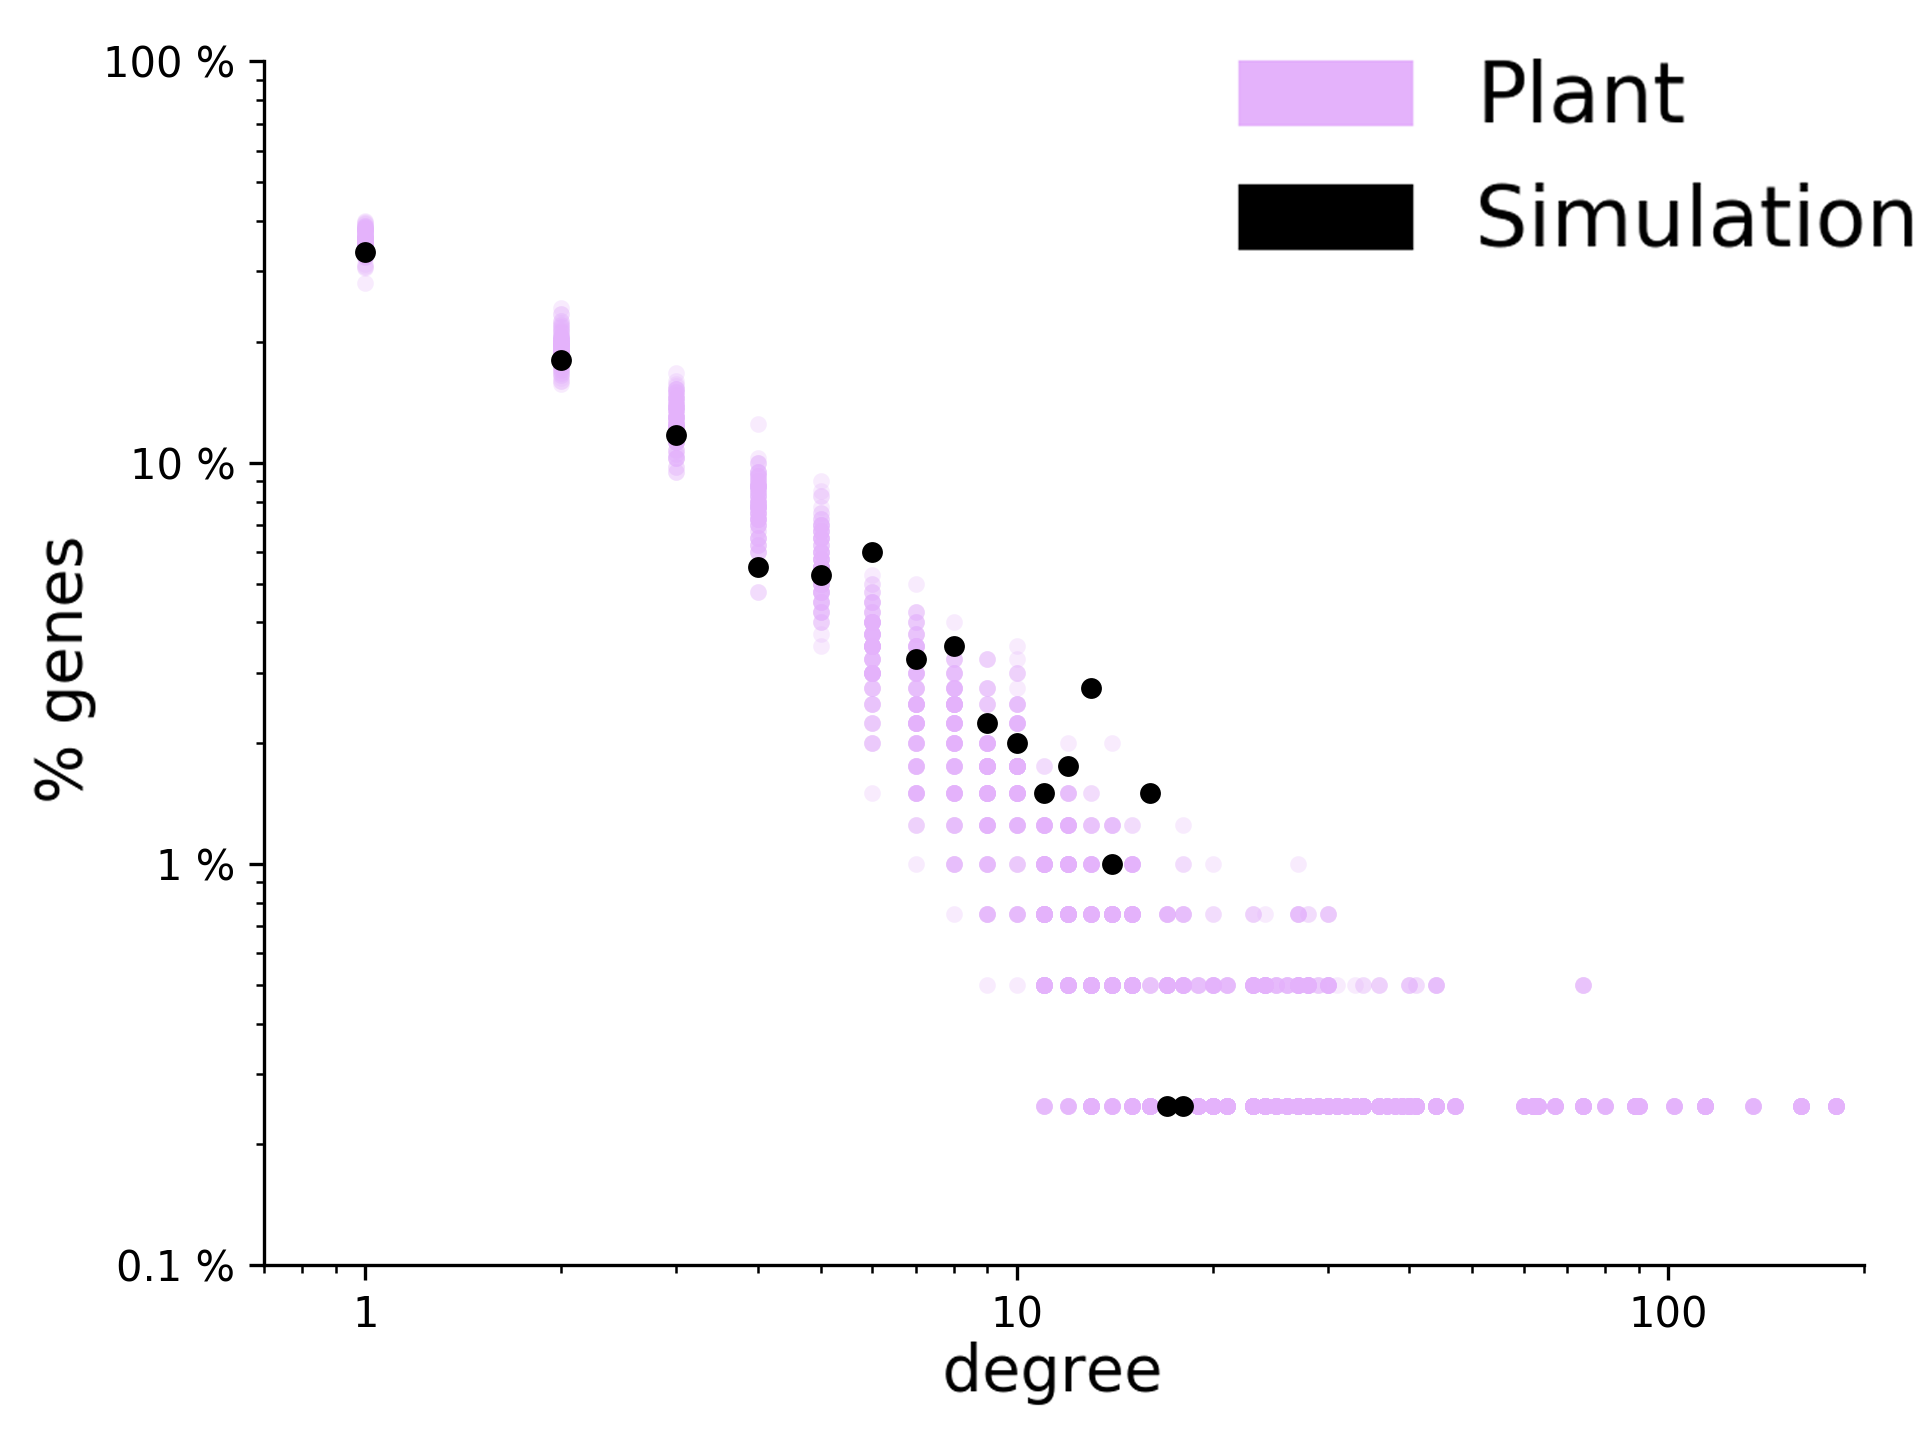
\includegraphics[scale=.36]{/adaptation_with_growth/faint_alpha/Evo_Plant.png}
		\caption{Adaptation with growth. Starting from a near empty network, evolution proceeds with mutations being random edge-reassignment  as 
		well as the addition of new nodes and edges. The size of the last network at algorithm termination is 400 nodes. The evolving networks 
		are not mutated with additional edges when their edge:node ratio exceeds that of the corresponding BN of the same edge:node ratio. 
		Shown here is the degree distribution of the fittest final network after 4000 generations of mutate-and-select (black dots), against the 
		degree distribution of 100 400-node randomly sampled subnetworks from each corresponding BN (colour dots). 
		In all cases, each evolved network's degree 
		distribution closely follows its corresponding BN of the same edge:node ratio.}
		\label{evol_figure} 
\end{figure*}	 

%\subsubsection{Scalability}\label{size_physio_context}

We considered whether the model can scale to larger networks
by allowing the simulation to continue until the simulated network's size is equal to 
that of the corresponding BN, in contrast to previously described simulations (Figures \ref{adap_fig} and \ref{evol_figure}) which terminated when networks' size reached 
400 nodes. 
We performed four experiments in which the simulated networks were allowed to grow to a size
equal to that of Bacteria, Worm, Bacteria Regulatory, or Mouse Regulatory networks (see Table \ref{networks_summary} for their corresponding number of nodes/edges). 
The four experiments show the scalability of the model to larger networks, with the latter two further showing its scalability to 
the regulatory context (as opposed to all other networks which represent protein-protein interactions). 
Figure \ref{large_PPI}  shows the degree distribution of the 
the fittest network after multiple generations of mutate-and-select. The number of generations is approximately equal to that of the number
of nodes in the corresponding BN. In contrast to the smaller-sized evolved networks depicted in Figure \ref{evol_figure}, 
the larger simulation networks shown in Figure \ref{large_PPI} show an even smoother distribution particularly of hubs of degree $\geq$10. 
%\begin{comment}
\begin{figure*}[h]
		\centering
		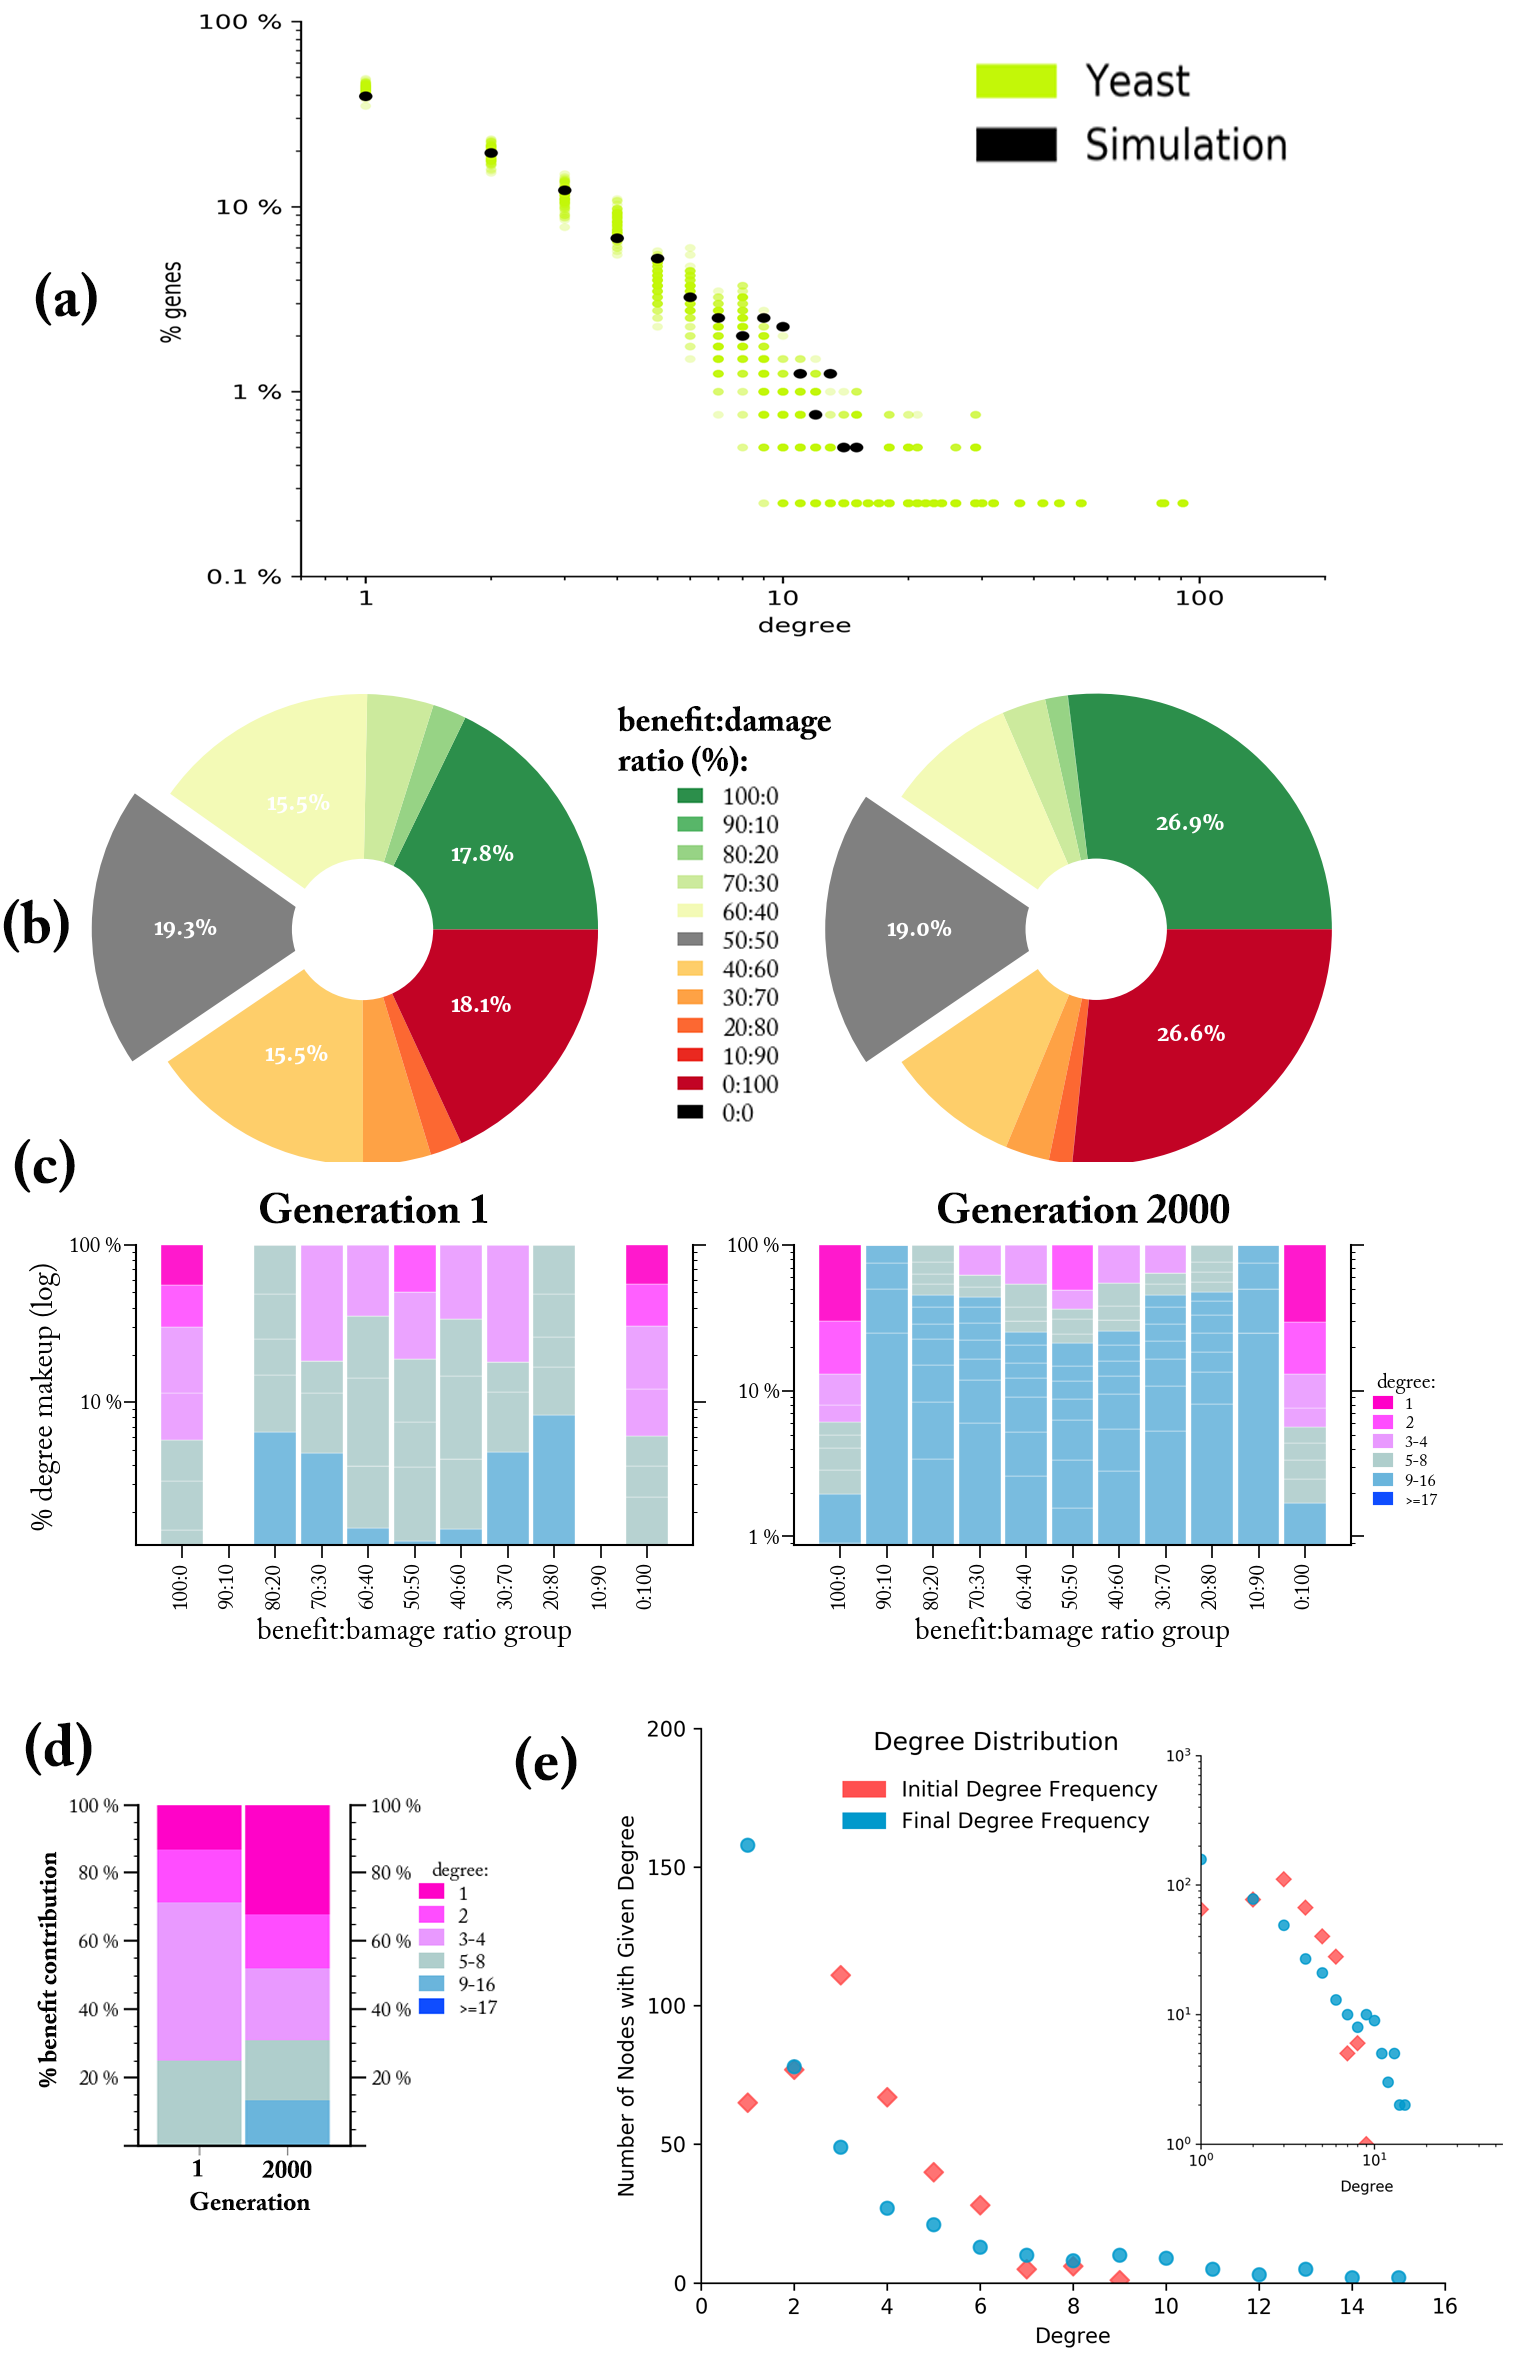
\includegraphics[width=17cm, height=10.5cm]{/results_additional/final/photoshop/processed.png}%origina ratio 1:0.77 width:height
		\caption{
				Scaling to larger networks and applicability to different physiological contexts. Networks start empty and undergo reassign-edge, add-node, 
				add-edge mutations. An evolving network grows by adding one node, and one or more edges while maintaining its edge:node ratio equal  
				that of its corresponding real BN. The simulation terminates when networks reach the same size (number of nodes) as that of the corresponding real BN. 
				The final 
				degree distribution of the fittest network is illustrated (horizontal black dashes) against that of the corresponding BN 
				(vertical coloured dashes). 
				Simulating against Bacteria and Mouse Regulatory networks (bottom row),  which are comprised of TF-gene, TF-TF and (in Mouse only) small RNA-gene 
				interactions as opposed to all 
				other networks which are comprised of protein-protein interactions, further shows the applicability of the model to different physiological contexts.
		}
		\label{large_PPI}
\end{figure*}	
%\end{comment}
	
		
		
\section{Methods}
The simulation begins with a random network of 400  (adaptation) or 4 (adaptation with growth) nodes . The number of edges is defined by the
 chosen edge:node ratio that matches that of a given BN. Each individual network in the population is mutated once per generation. Mutation involves 
 removing one randomly selected edge and replacing it with another edge between two random nodes.
 The interaction sign (promotional or inhibitory) is also assigned at random. 
 The network must remain connected, meaning that no edge is removed if it severs one section of the network from the rest. 
 After mutation, each network is assessed based on a number of NEP instances that is either fixed at 100 for the 400-node simulations, or varied proportional to ${\sim}$
 10\% of the total nodes in the network for simulation of larger networks (Figure \ref{large_PPI}). 
 For extremely small networks at early generations of adaptation-with-growth simulations of larger networks, a minimum 
 of 10 NEP instances was generated. 
 The threshold  of tolerated damaging interactions 
 in the solution 
 is imposed at 5\% of the sum of all damages in all simulations. The top 10\% fittest networks represent the surviving population and 
 are used to spawn the population of networks for the next generation by making an equal number of exact replicas from each of the four. 
 The population size is kept constant at 40-64 networks throughout the generations. 
 
 For the adaptation-with-growth simulations  (Section \ref{evolution_results}), a random node is added every 5 generations (in the 400-node networks
 shown in Figures \ref{adap_fig} and \ref{evol_figure}) 
 or at every generations  (full-network simulations shown in Figure \ref{large_PPI}). 
 In addition,  the appropriate number of edges are added to maintain the  edge:node ratio of the corresponding BN. The simulation 
 proceeds to evolve for 2000 generations or until the desired network size is reached. 
 In simulations where network size is capped at 400 nodes, the algorithm continues to evolve for 2000 more generations 
 but with edge-reassignment mutation only. NEP instances were reduced to knapsack instances \cite{atiia_computational_2017-1} 
 and solved to optimality using a pseudopolynomial algorithm \cite{pisinger_where_2005} 
 implemented in C. Networks were encoded and manipulated using the NetworkX package \cite{schult_exploring_2008}.
 \begin{comment}
 The Bacteria Regulatory network was extract from RegulonDB \cite{gama-castro_regulondb_2016} 
 with interactions that meet have the following properties:(1) Experimentally-validated (as opposed to computationally-predicted), 
(2) Have "Strong" or "Confirmed" evidence (as opposed to "Weak"), (3) Randomized +/- interaction effect (promotional/inhibitory) in
 cases where the RegulonDB designates it as "?" (unknown) or +/- (dual), 
(4) Interactions are between transcription factor (TF)-Gene, TF-TF (non of small RNA (sRNA) -Gene interactions have "Strong" or 
"Confirmed" evidence so there were excluded\footnote{\scriptsize{ see http://regulondb.ccg.unam.mx/menu/download/datasets/files/sRNABindingSiteSet.txt}}, 
(5) Interactions involving Sigma proteins are not included since they are very common to all transcriptions and therefore do not in and of themselves control the combinatorial regulatory state of the organism, and 
(6) In cases where an interaction was reported more than once, and the reported sign doesn't agree, the sign is randomized with more likelihood proportional to the number of times it was reported (e.g. if a reaction was reported four times and the signs were [+ + + -] were reported, a '+' is chosen with  75\% chance. 
All other networks represent (undirected) protein-protein networks and were taken as is from their respective sources. 
\end{comment}
\begin{comment}
Synthetic networks are simulated using a genetic algorithm. Individuals in the population are gene interaction networks. Variation is 
generated through mutation that only affects network connectivity by altering edges. Fitness is determined based on the computational 
ease of the NEP instances that the network yields. Only the fittest networks survive and copy themselves to form a new population of 
networks. The process repeats for many generations.
The simulation begins with a random Erdos-Renyi network with 400 nodes. Every pair of nodes has a .005 chance of acquiring an edge, 
which results in a mean of 800 edges. Each edge is randomly assigned a qualitative sign to represent a promoting or inhibiting interaction. 
The initial network is assessed based on many NEP instances, as described below. The fitness and degree distribution are recorded. 
The simulation proceeds to evolve for 4000 generations. At each generation a population of 40 networks is generated from exact replicates 
of the surviving population. At the first generation this is simply the initial Erdos-Renyi network. Each network in the population is 
mutated and then assigned a fitness score based on the NEP instances it yields. 
Mutation involves removing one randomly selected edge and replacing it with another edge between two random nodes with a random interaction sign. 
In doing so the number of edges is conserved and only the connectivity is altered. Moreover, the network must remain connected, meaning that no 
edge is removed if it severs one section of the network from the rest. Mutation begins with 4 replacements per generation for each individual 
in the population and slows down in a linear fashion until it reaches one mutation per generation.
After mutation, each network is assessed based on 400 NEP instances. Many instances are used to assess the network’s ability to adapt to an 
arbitrary environment, rather than a specific condition. An oracle advice is generated with the ideal interaction sign for each edge of the 
network. If the network’s edge matrix matches the advice, the two nodes of that edge acquire a benefit. Otherwise, they both incur a damage. 
The reduction is not specific to the direction of the edge, since the loss of either gene would nullify the interaction. The benefits and 
damages are used to reverse-reduce to the knapsack problem. The number of tolerated damages (knapsack capacity) is 10\% of the sum of all damages.
The knapsack instance is scored based on its ability to circumvent computational intractability. The network fitness is the average of 
its 400 instance scores. The fittest network in the population outputs its fitness score and degree distribution. The top 4 fittest 
networks comprise the surviving population and are used to spawn the population of networks for the next generation.
\end{comment}
\section{Discussion}
Our simulation results show that computational intractability provides sufficient conditions for the emergence of the majority-leaves minority-hubs (mLmH) topology, irrespective of whether it follows a power-law distribution in a technical sense as has previously been intensely debated (see \cite{lima-mendez_powerful_2009} and references therein). The fact that the intractability of NP-hard problems is (assuming P$\neq$NP) universally insurmountable renders it a necessary condition as well: it rules out the possibility of any other topology. A completely sparse network where each gene has only one interaction produces the easiest possible optimization instances (every gene can unambiguously be either beneficial or detrimental under any evolutionary pressure scenario). However, it also leads to a need for more genes since functions that could have been handled by one hub gene of degree $d$ must now be handled by $d$ specialty genes. This obviously leads to an explosion of genome size. Conversely, a highly dense network where the number of genes is minimized and interactions are handled by multi-purpose hub genes leads to an exponential search space: the number of iterations of random-variations and non-random selection \cite{carvunis_proto-genes_2012} before the network has been optimally rewired into a healthier state (i.e. the right subset genes has been conserved, discovered, mutated or deleted to overcome a given evolutionary pressure)  would be exponential in network size. The majority-leaves minority-hubs topology is the middle ground between these two extremes: concentrate essential functions in hubs genes \cite{gerstein_architecture_2012}, and respond to evolutionary pressure by experimenting (on the cheap) with loosely connected leaf genes at the periphery of the network \cite{kim_positive_2007}. Highly connected genes tend to perform essential functions \cite{khurana_interpretation_2013} and are unlikely to be detrimental in and of themselves. Regulating around them however (e.g. micro-RNA regulation \cite{gerstein_architecture_2012}) is where the constant optimization is needed. 
%NP-hardness is universally insurmountable, but what guarantee is there that the network evolution problem, as we defined it, captures the optimization dilemma of evolving systems? 

For the presented model to be applicable beyond explaining the emergence of mLmH, some limitations must be addressed. 
%The model presented here is not without limitations. 
We have treated all interactions (edges) as equal, but in reality some interactions are more potent than others. Unfortunately there is no large-scale data as of yet that can inform meaningful assignment of edge weights (i.e. some $\pm \alpha\in \mathbb{R}$ instead of simply $\pm$1). Alternatively potency can be estimated based on the centrality  of a given interaction (how many network shortest paths include it).  We have also treated all genes (nodes) as equal, but in reality a gene's position matters \cite{kim_positive_2007,gerstein_architecture_2012} and should be taken into account when attributing the magnitude of its benefit/damage scores. The benefit(damage) score of a central gene (many shortest paths pass through it) clearly has more positive (negative) impact on the network as a whole. Future work aims to overcome these limitations and apply its simulations as stress tests on experimentally-validated networks the coverage and accuracy of which is exponentially increasing \cite{han_trrust:_2015, neph_circuitry_2012, gerstein_architecture_2012, stergachis_conservation_2014}. In this regard, we intend to ask the following question: what subset of pathways are involved in the hardest optimization instances under simulated evolutionary pressure? If the quick sands of computational intractability is the obstacle against Nature discovering a cancer-resistant regulatory network for example, the model may give a hint as to what subset of genes should combinatorially be optimized over (up- and down-regulation of genes). This can inform knockdown/out/in and RNA interference experiments, and is in sharp contrast with the dominant correlation-based cancer-target inference methods which, even if statistically sound, do not necessarily reveal underlying causation. The efficacy of the model in making such predictions can easily be falsified against previously known cancer-implicated sets of genes. 
% from the ENCODE paper "Architecture of the human regulatory network derived from ENCODE data": 
% Highly connected network elements (both transcription factors and targets) are under strong evolutionary 
% selection and exhibit stronger allele-specific activity (this is particularly apparent when multiple factors are involved). 
%Surprisingly, however, elements with allelic activity are under weaker selection than non-allelic ones.
%  *** see also the child notes for this paper in Zotero

\begin{acks} 
	Computations were made on the supercomputing cluster Guillimin from McGill University, managed by Calcul Québec and Compute Canada. The operation of these supercomputers is funded by the Canada Foundation for Innovation (CFI), ministère de l’Économie, de la Science et de l’Innovation du Québec (MESI) and the Fonds de recherche du Québec - Nature et technologies (FRQ-NT).
\end{acks}

\bibliographystyle{ACM-Reference-Format}
%\balance
\bibliography{/Users/mohammedalshamrani/Downloads/School/Waldispul/Publishing/z-misc/zotero-library/better_bibtex} 
\balance
\end{document}
